\documentclass[11pt,a4paper,oneside]{report}
% Preambul comun (documentație + prezentare folosesc aceleași figuri).
\usepackage{fontspec}
\usepackage[romanian]{babel}
\usepackage{csquotes}
\usepackage{newunicodechar}
% Simboluri absente din Latin Modern: le compunem în modul matematic.
\newunicodechar{≈}{\ensuremath{\approx}}
\newunicodechar{≤}{\ensuremath{\leq}}
\newunicodechar{≥}{\ensuremath{\geq}}
\newunicodechar{↔}{\ensuremath{\leftrightarrow}}
\usepackage{amsmath,amssymb}
\usepackage{xcolor}
\usepackage{tikz}
\usetikzlibrary{arrows.meta,positioning,shapes.geometric,shapes.multipart,fit,backgrounds,calc,decorations.pathreplacing,matrix}
\usepackage{pgfplots}
\pgfplotsset{compat=1.18}
% Format numeric românesc pe axe: 60.000 și 0,8.
\pgfkeys{/pgf/number format/.cd, use comma, 1000 sep={.}}
\usepgfplotslibrary{groupplots}

% Paletă (accesibilă, distinctă în alb-negru prin marcaje).
\definecolor{c1}{HTML}{2F6FDE}
\definecolor{c2}{HTML}{E07B39}
\definecolor{c3}{HTML}{1F9D63}
\definecolor{c4}{HTML}{8E5CC4}
\definecolor{c5}{HTML}{C8423B}
\definecolor{c6}{HTML}{6B7280}
\definecolor{boxbg}{HTML}{F3F5F9}

\pgfplotscreateplotcyclelist{spd}{
  {c1,mark=*,thick},{c2,mark=square*,thick},{c3,mark=triangle*,thick},
  {c4,mark=diamond*,thick},{c5,mark=pentagon*,thick},{c6,mark=o,thick,dashed}}
\pgfplotsset{
  every axis/.append style={cycle list name=spd, grid=major, grid style={gray!25},
    tick label style={font=\footnotesize}, label style={font=\small},
    legend style={font=\footnotesize, draw=none, fill=white, fill opacity=0.85, text opacity=1},
    legend cell align=left},
}

% Axe de debit în mii: 60k în loc de 60.000.
\pgfplotsset{kticks/.style={scaled y ticks=base 10:-3, ytick scale label code/.code={},
  yticklabel={\pgfmathprintnumber[fixed,precision=0]{\tick}k}}}

\tikzset{
  comp/.style={draw, rounded corners=3pt, fill=boxbg, minimum height=8mm, minimum width=22mm, align=center, font=\small},
  store/.style={draw, cylinder, shape border rotate=90, aspect=0.25, fill=boxbg, minimum height=11mm, minimum width=18mm, align=center, font=\small},
  arr/.style={-{Stealth[length=2.2mm]}, thick},
  darr/.style={{Stealth[length=2.2mm]}-{Stealth[length=2.2mm]}, thick},
  note/.style={font=\scriptsize, text=black!65, align=center},
}

\usepackage[margin=2.5cm]{geometry}
\usepackage{microtype}
\usepackage{booktabs,tabularx,array}
\usepackage{caption,subcaption}
\usepackage{float,placeins}
\usepackage{enumitem}
\usepackage{listings}% doar pentru tipul de float/caption „Listing”
\usepackage{fancyvrb}
% fancyvrb suportă UTF-8 în LuaLaTeX (listings reordonează diacriticele).
\newenvironment{code}[1]{%
  \par\def\codecap{#1}\ifx\codecap\empty\else\captionof{lstlisting}{#1}\fi
  \VerbatimEnvironment
  \begin{tcolorbox}[colback=codebg, colframe=gray!30, boxrule=0.4pt, arc=1pt, left=3pt, right=3pt, top=1pt, bottom=1pt]
  \begin{Verbatim}[fontsize=\footnotesize]}
  {\end{Verbatim}\end{tcolorbox}}
\usepackage{fancyhdr}
\usepackage{titlesec}
\usepackage[most]{tcolorbox}
\usepackage[hidelinks]{hyperref}
\usepackage[nameinlink]{cleveref}
% cleveref nu are traducere în română.
\crefname{chapter}{capitolul}{capitolele}\Crefname{chapter}{Capitolul}{Capitolele}
\crefname{section}{secțiunea}{secțiunile}\Crefname{section}{Secțiunea}{Secțiunile}
\crefname{figure}{figura}{figurile}\Crefname{figure}{Figura}{Figurile}
\crefname{table}{tabelul}{tabelele}\Crefname{table}{Tabelul}{Tabelele}
\crefname{equation}{relația}{relațiile}\Crefname{equation}{Relația}{Relațiile}
\crefname{appendix}{anexa}{anexele}\Crefname{appendix}{Anexa}{Anexele}
\crefname{lstlisting}{listingul}{listingurile}\Crefname{lstlisting}{Listingul}{Listingurile}

\setmainfont{Latin Modern Roman}
\setmonofont{Latin Modern Mono}[Scale=0.95]
\setlist{itemsep=2pt, topsep=4pt}
\captionsetup{font=small, labelfont=bf}
\titleformat{\chapter}[hang]{\Huge\bfseries}{\thechapter\hspace{12pt}\textcolor{c1}{|}\hspace{12pt}}{0pt}{\Huge\bfseries}
\pagestyle{fancy}\fancyhf{}\fancyhead[L]{\small\leftmark}\fancyfoot[C]{\thepage}
\renewcommand{\headrulewidth}{0.3pt}

\definecolor{codebg}{HTML}{F6F8FA}
\lstdefinelanguage{Rust}{
  keywords={fn,let,mut,pub,struct,enum,impl,match,if,else,for,in,while,loop,return,async,await,move,use,mod,crate,self,Self,where,trait,type,const,static,as,ref,Some,None,Ok,Err,true,false},
  sensitive=true, comment=[l]{//}, morestring=[b]"}
\lstset{basicstyle=\ttfamily\footnotesize, backgroundcolor=\color{codebg}, frame=single, rulecolor=\color{gray!30},
  keywordstyle=\color{c1}\bfseries, commentstyle=\color{c3}\itshape, stringstyle=\color{c2},
  breaklines=true, columns=fullflexible, keepspaces=true, xleftmargin=4pt, xrightmargin=4pt}

\newtcolorbox{ideea}[1][]{colback=c1!5, colframe=c1!60, fonttitle=\bfseries\small, title={#1}, boxrule=0.6pt, arc=2pt}

% Date de identificare — completează după caz.
\newcommand{\Universitate}{Universitatea \textit{(de completat)}}
\newcommand{\Facultate}{Facultatea \textit{(de completat)}}
\newcommand{\Program}{Master — Proiect individual: aplicații paralele și distribuite}
\newcommand{\Autor}{Cristi Miloiu}

\newcommand{\datadir}{data/}
% Rezultatele experimentale (generate de scripts/plots_data.py din results/*.csv).
\InputIfFileExists{data/numbers.tex}{}{}

\begin{document}

\begin{titlepage}
  \centering
  {\large \Universitate\\ \Facultate\\[2pt] \Program\par}
  \vspace{3.2cm}
  {\Huge\bfseries Aplicație de tip memory cache\\[4pt] pentru aplicații web\par}
  \vspace{0.8cm}
  {\Large Implementare folosind tabele in-memory și o bază de date relațională.\\ Evaluarea performanțelor\par}
  \vspace{1.6cm}
  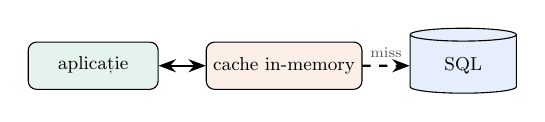
\begin{tikzpicture}[scale=0.75, transform shape]
    \node[comp, fill=c3!12] (a) {aplicație};
    \node[comp, fill=c2!12, right=8mm of a] (c) {cache in-memory};
    \node[store, fill=c1!12, right=8mm of c] (d) {SQL};
    \draw[darr] (a) -- (c); \draw[arr, dashed] (c) -- node[note, above] {miss} (d);
  \end{tikzpicture}
  \vfill
  {\large Document de analiză și proiectare\par}
  \vspace{0.4cm}
  {\large Student: \Autor\par}
  \vspace{0.3cm}
  {\large \today\par}
\end{titlepage}

\begin{abstract}
\noindent
Lucrarea prezintă proiectarea, implementarea și evaluarea experimentală a unui sistem de cache in-memory
pentru aplicații web, scris integral în Rust. Componenta centrală este \texttt{memtable}, un motor de
tabele in-memory cu \emph{sharding}, politici de evacuare LRU/FIFO/CLOCK, expirare TTL și invalidare pe
etichete. Motorul este folosit atât în procesul aplicației (cache local L1), cât și într-un cluster de
noduri distribuite, adresate prin \emph{consistent hashing}. Sursa de adevăr este o bază de date
relațională PostgreSQL; coerența cache-urilor locale ale mai multor instanțe se obține prin
mecanismul \texttt{LISTEN/NOTIFY}. Aplicația web (axum + tokio) permite comutarea la runtime între șase
backend-uri (fără cache, local, cluster, near-cache pe două niveluri, Redis și o tabelă
\texttt{UNLOGGED} într-un PostgreSQL ținut în RAM) și trei strategii de scriere (invalidare,
write-through, write-behind), ceea ce face posibilă compararea lor în condiții identice. Întregul sistem
— două instanțe web în spatele unui load balancer, trei noduri de cache, Redis, două servere
PostgreSQL, Prometheus și Grafana — rulează cu Docker Compose. Evaluarea cuprinde opt experimente
HTTP și două benchmark-uri offline, care măsoară debitul, latența (p50/p95/p99), rata de hit,
scalabilitatea cu numărul de fire, de clienți, de instanțe și de noduri, precum și efectul protecției
împotriva \emph{cache stampede}.
\end{abstract}

\tableofcontents

\chapter{Introducere}
\label{ch:intro}

\section{Context și motivație}

Aplicațiile web moderne servesc un volum mare de cereri de citire asupra unor date relativ
stabile: pagini de produs, profile, clasamente, configurații. Baza de date relațională rămâne sursa
de adevăr datorită garanțiilor tranzacționale (ACID), dar fiecare interogare implică rețea,
analiză sintactică, planificare, acces la pagini și eventual agregări costisitoare. Atunci când
aceeași informație este cerută de mii de ori pe secundă, recalcularea ei la fiecare cerere este
risipă de resurse și, mai ales, sursă de latență.

Un \emph{cache in-memory} păstrează rezultate deja calculate în memoria RAM, aproape de aplicație,
astfel încât cererile repetate să fie servite în microsecunde, fără a atinge baza de date. Practic
toate sistemele web la scară mare folosesc o astfel de soluție (Memcached la Facebook
\cite{memcache-fb}, Redis, cache-uri locale de tip Caffeine/Guava etc.). Problema este însă mai
subtilă decât pare: memoria este limitată (trebuie ales \emph{ce} păstrăm), datele se modifică
(trebuie menținută coerența), iar sistemul este distribuit (mai multe instanțe, mai multe noduri).

\section{Obiectivele proiectului}

Proiectul urmărește proiectarea și realizarea unei aplicații paralele și distribuite care să răspundă
concret acestor probleme:

\begin{enumerate}
  \item un \textbf{motor de tabele in-memory} (\texttt{memtable}) thread-safe, cu sharding, politici de
        evacuare LRU/FIFO/CLOCK, TTL și invalidare pe grupuri de chei (tag-uri);
  \item un \textbf{cache distribuit}: noduri de cache accesate printr-un protocol TCP propriu și un client
        care distribuie cheile prin \emph{consistent hashing};
  \item o \textbf{aplicație web} realistă (catalog de produse cu recenzii în PostgreSQL) care folosește
        cache-ul prin mai multe strategii de citire și scriere, comutabile la runtime;
  \item \textbf{comparația cu alternative}: Redis și o tabelă in-memory relațională (tabelă
        \texttt{UNLOGGED} într-un PostgreSQL cu date pe \texttt{tmpfs});
  \item o \textbf{evaluare experimentală} riguroasă: debit, latențe pe percentile, rata de hit,
        scalabilitate (fire, clienți, instanțe, noduri) și comparația cu varianta secvențială.
\end{enumerate}

\section{Contribuții}

\begin{itemize}
  \item Implementare completă în Rust (≈3.400 de linii), fără cod \texttt{unsafe}, verificată cu
        \texttt{clippy} în modul \emph{pedantic} și acoperită de teste unitare și de integrare.
  \item Infrastructură reproductibilă cu Docker Compose: 12 containere, observabilitate cu
        Prometheus și Grafana, documentație OpenAPI (Swagger) și o interfață web de control.
  \item Mecanisme avansate: \emph{single-flight} (protecție la \emph{cache stampede}), cache pe două
        niveluri (\emph{near-cache}), invalidare distribuită prin \texttt{LISTEN/NOTIFY}, write-behind cu
        grupare în loturi și oprire fără pierderi de date.
  \item Un generator de încărcare propriu cu distribuție Zipf și histograme HDR și un simulator
        trace-driven pentru politicile de evacuare, comparate cu limita teoretică.
\end{itemize}

\section{Structura documentului}

\Cref{ch:fundamente} prezintă fundamentele teoretice. \Cref{ch:analiza} definește problema și
cerințele și compară arhitectura secvențială cu cea paralelă/distribuită. \Cref{ch:arhitectura}
descrie arhitectura sistemului, iar \cref{ch:implementare} detaliile de implementare.
\Cref{ch:tehnologii} trece în revistă tehnologiile utilizate. \Cref{ch:evaluare} conține
metodologia și rezultatele experimentale, iar \cref{ch:concluzii} concluziile. Anexa
\ref{ch:rulare} descrie rularea proiectului.

\chapter{Fundamente teoretice}
\label{ch:fundamente}

\section{Ierarhia de memorie și localitatea referințelor}

Ideea de cache provine din arhitectura calculatoarelor: o memorie mică și rapidă păstrează o
submulțime a datelor dintr-o memorie mare și lentă \cite{hennessy}. Eficiența ei se bazează pe
\emph{localitatea referințelor}: datele accesate recent (localitate temporală) sau populare vor fi
probabil accesate din nou. În aplicațiile web, ierarhia arată astfel:

\begin{table}[H]
\centering\small
\begin{tabular}{lll}
\toprule
Nivel & Exemplu & Latență tipică \\
\midrule
Memorie în proces (L1) & \texttt{HashMap} protejat de mutex & 0{,}05–1 µs \\
Cache în rețea locală (L2) & Memcached, Redis, \texttt{cache-node} & 50–300 µs \\
Bază de date, date în RAM & PostgreSQL, \emph{shared buffers} & 0{,}2–2 ms \\
Bază de date, agregări / disc & join + \texttt{GROUP BY}, I/O & 2–100 ms \\
\bottomrule
\end{tabular}
\caption{Ordine de mărime ale latențelor în ierarhia de date a unei aplicații web.}
\end{table}

Timpul mediu de acces efectiv este dat de relația clasică:
\begin{equation}
  T_{\text{mediu}} = h \cdot T_{\text{cache}} + (1-h)\cdot\left(T_{\text{cache}} + T_{\text{DB}}\right)
  = T_{\text{cache}} + (1-h)\cdot T_{\text{DB}},
  \label{eq:amat}
\end{equation}
unde $h$ este rata de hit. Deoarece $T_{\text{DB}} \gg T_{\text{cache}}$, câștigul este dominat de
$(1-h)$: trecerea de la $h=0{,}90$ la $h=0{,}99$ reduce de zece ori numărul de accesări ale bazei de
date. Rata de hit este deci metrica centrală a oricărui cache.

\section{Distribuția Zipf a popularității}

Studiile asupra traficului web \cite{breslau} arată că popularitatea obiectelor urmează aproximativ o
lege Zipf: probabilitatea ca o cerere să vizeze obiectul de rang $i$ dintr-un total de $N$ este
\begin{equation}
  p_i = \frac{i^{-s}}{H_{N,s}}, \qquad H_{N,s} = \sum_{k=1}^{N} k^{-s},
\end{equation}
unde exponentul $s$ (de obicei între $0{,}6$ și $1{,}2$) controlează asimetria. În modelul
\emph{Independent Reference Model} (IRM), cel mai bun cache static de capacitate $C$ păstrează cele
mai populare $C$ obiecte și atinge rata de hit
\begin{equation}
  h^{*}(C) = \frac{H_{C,s}}{H_{N,s}},
  \label{eq:ideal}
\end{equation}
care este o limită superioară utilă pentru politicile reale (folosită în \cref{sec:sim}). Pentru
$s = 0{,}99$ și $N = 100.000$, un cache cu doar 10\% din chei poate servi teoretic aproape 80\% din
cereri — de aici eficiența cache-urilor mici.

\section{Politici de evacuare}

Când cache-ul este plin, trebuie ales ce intrare se elimină. Algoritmul optim (Belady, MIN)
\cite{belady} elimină intrarea care va fi folosită cel mai târziu în viitor, dar necesită cunoașterea
viitorului. Politicile practice aproximează acest comportament:

\begin{description}
  \item[FIFO] elimină cea mai veche intrare inserată; ignoră complet accesele. Cost minim, rată de hit
        mai slabă.
  \item[LRU] (\emph{Least Recently Used}) elimină intrarea neaccesată de cel mai mult timp. Exploatează
        localitatea temporală, dar fiecare acces modifică structura (mutare în capul listei), ceea ce
        crește contenția sub concurență. Este vulnerabilă la \emph{scanări}: o parcurgere secvențială a
        multor chei reci elimină setul fierbinte.
  \item[CLOCK] (\emph{second chance}) \cite{corbato} aproximează LRU cu un singur bit de referință per
        intrare: la acces doar se setează bitul; la evacuare, intrările cu bitul setat primesc o „a doua
        șansă" (bitul se resetează). Accesul nu mai mută noduri, deci operația de citire este mai ieftină.
\end{description}

Politici mai sofisticate (LFU, ARC \cite{megiddo}, W-TinyLFU) combină recența cu frecvența; ele sunt
discutate ca direcții viitoare.

\section{Strategii de citire și scriere}

\paragraph{Cache-aside (lazy loading).} Aplicația caută întâi în cache; la \emph{miss} citește din baza
de date și populează cache-ul. Este modelul folosit pentru citiri în acest proiect.

\paragraph{Invalidare la scriere.} La o modificare, aplicația scrie în baza de date și apoi
\emph{șterge} intrarea din cache. Este simplă și sigură, dar următoarea citire va fi un miss.

\paragraph{Write-through.} Aplicația scrie în baza de date și apoi \emph{actualizează} cache-ul cu
valoarea nouă. Rata de hit se păstrează, cu prețul unei latențe de scriere mai mari.

\paragraph{Write-behind (write-back).} Aplicația actualizează imediat cache-ul și confirmă clientul;
scrierea în baza de date este amânată și grupată în loturi. Scrierile devin foarte rapide și numărul de
tranzacții scade drastic, dar consistența devine \emph{eventuală}, iar o cădere înainte de flush poate
pierde date.

\section{Consistență și coerență}

Un cache introduce inevitabil o a doua copie a datelor. Teorema CAP \cite{brewer} formalizează
compromisul dintre consistență și disponibilitate în prezența partițiilor de rețea; pentru cache-uri,
alegerea uzuală este \emph{consistența eventuală} cu fereastră de inconsistență limitată de TTL.
Probleme clasice:

\begin{itemize}
  \item \textbf{coerența cache-urilor locale}: fiecare instanță are propria copie; o scriere pe instanța A
        trebuie să invalideze copia din B. Proiectul folosește notificări \texttt{LISTEN/NOTIFY} emise de
        un trigger PostgreSQL.
  \item \textbf{cursa citire–invalidare}: un cititor obține valoarea veche din DB, un scriitor modifică și
        invalidează, apoi cititorul populează cache-ul cu valoarea veche. TTL-ul limitează durata
        inconsistenței; soluții complete folosesc \emph{lease}-uri \cite{memcache-fb} sau versiuni.
  \item \textbf{cache stampede} (\emph{thundering herd}): la expirarea unei chei foarte populare, sute de
        cereri concurente ratează simultan și lovesc baza de date. Soluția implementată este
        \emph{single-flight}: o singură cerere per cheie interoghează baza de date, celelalte așteaptă
        rezultatul.
\end{itemize}

\section{Distribuirea datelor: consistent hashing}

Distribuirea cheilor pe $n$ noduri prin $\text{hash}(k) \bmod n$ este echilibrată, dar la adăugarea unui
nod aproape toate cheile își schimbă nodul, ceea ce golește efectiv cache-ul. \emph{Consistent hashing}
\cite{karger} plasează nodurile și cheile pe un inel; fiecare cheie aparține primului nod întâlnit în
sens orar. La modificarea topologiei se mută doar $\approx 1/n$ din chei. Pentru echilibrare, fiecare nod
fizic apare de mai multe ori pe inel (\emph{noduri virtuale}).

\section{Metrici și legi de performanță}

\paragraph{Legea lui Little.} Pentru un sistem stabil, numărul mediu de cereri în sistem este
$L = \lambda W$ \cite{little}. Într-un test \emph{closed-loop} cu $L$ clienți concurenți, debitul este
$\lambda = L / W$: dacă latența rămâne constantă, debitul crește liniar cu concurența, până la saturarea
unei resurse.

\paragraph{Legea lui Amdahl.} Dacă o fracțiune $f$ a lucrului este paralelizabilă, accelerarea maximă pe
$p$ procesoare este \cite{amdahl}
\begin{equation}
  S(p) = \frac{1}{(1-f) + f/p}.
  \label{eq:amdahl}
\end{equation}
Secțiunile critice (de exemplu un mutex global) reprezintă partea serială $(1-f)$; sharding-ul reduce
această parte.

\paragraph{Percentile de latență.} Media ascunde coada distribuției. Pentru aplicații web contează p95,
p99 și p99.9: cu 100 de apeluri per pagină, aproape fiecare pagină „vede" latența p99. Latențele sunt
înregistrate cu histograme HDR \cite{tene}, cu precizie de 3 cifre semnificative.

\chapter{Analiza problemei}
\label{ch:analiza}

\section{Definirea problemei}

Se consideră un magazin online cu \textbf{200 de categorii}, \textbf{100.000 de produse} și
\textbf{500.000 de recenzii}, stocate în PostgreSQL. Aplicația web expune trei operații:

\begin{enumerate}
  \item \texttt{GET /api/products/\{id\}} — detaliile unui produs împreună cu media notelor și numărul de
        recenzii (în forma normalizată: \texttt{LEFT JOIN} + agregare pe $\approx 5$ rânduri);
  \item \texttt{GET /api/categories/\{id\}/top} — cele mai bine cotate produse dintr-o categorie
        (în forma normalizată: \texttt{JOIN} + \texttt{GROUP BY} + sortare peste $\approx 2.500$ de rânduri);
  \item \texttt{PUT /api/products/\{id\}} — modificarea prețului și/sau stocului.
\end{enumerate}

Traficul este dominat de citiri (90–99\%), cu popularitate Zipf. Problema este: \emph{cum poate fi
servit acest trafic cu debit maxim și latență minimă, păstrând datele corecte, folosind memorie
limitată și mai multe mașini?}

\section{Cerințe}

\subsection{Cerințe funcționale}
\begin{itemize}
  \item F1. Citirea produselor și a clasamentelor, cu indicarea sursei (\texttt{X-Cache: HIT/MISS}).
  \item F2. Modificarea produselor, cu propagarea corectă în cache conform strategiei alese.
  \item F3. Comutarea la runtime a backend-ului de cache, a strategiei, politicii, capacității și TTL-ului.
  \item F4. Statistici: hit/miss, interogări DB, mărimea cozii write-behind, statistici per nod.
  \item F5. Documentație interactivă a API-ului (OpenAPI/Swagger) și o interfață de control.
\end{itemize}

\subsection{Cerințe nefuncționale}
\begin{itemize}
  \item N1. \textbf{Performanță}: latență p50 sub 1 ms pentru hit-uri; debit de ordinul zecilor de mii de
        cereri/s pe un singur host.
  \item N2. \textbf{Scalabilitate}: adăugarea de instanțe web și de noduri de cache crește capacitatea.
  \item N3. \textbf{Coerență}: o scriere confirmată trebuie să fie vizibilă pe toate instanțele în cel mult
        câteva sute de milisecunde (strategiile sincrone) sau după flush (write-behind).
  \item N4. \textbf{Reziliență}: căderea cache-ului nu trebuie să oprească aplicația (degradare la DB);
        oprirea aplicației nu trebuie să piardă scrierile din coada write-behind.
  \item N5. \textbf{Reproductibilitate}: întregul mediu pornește cu o singură comandă; experimentele sunt
        scriptate.
\end{itemize}

\section{Arhitectura secvențială}
\label{sec:secvential}

Varianta de referință (\cref{fig:seqpar}a) este un singur proces care tratează cererile una câte una și
interoghează baza de date pentru fiecare citire. Analiza ei arată limitele:

\begin{itemize}
  \item debitul este $\lambda = 1/W$, unde $W$ include rețeaua și execuția interogării; cu $W \approx 1$ ms
        obținem cel mult $\approx 1.000$ cereri/s, indiferent de numărul de nuclee disponibile;
  \item baza de date este solicitată de fiecare cerere, deși 80–90\% dintre cereri vizează aceleași câteva
        mii de obiecte;
  \item nu există toleranță la defecte: căderea procesului oprește serviciul.
\end{itemize}

Varianta secvențială este reprodusă experimental prin backend-ul \texttt{none} cu un singur client
(experimentul E4, concurență 1) și, pentru motorul de cache, prin configurația 1 fir × 1 shard.

\section{Arhitectura paralelă și distribuită}
\label{sec:paralel}

\begin{figure}[H]
  \centering
  \resizebox{0.95\linewidth}{!}{% Arhitectura secvențială vs paralelă/distribuită.
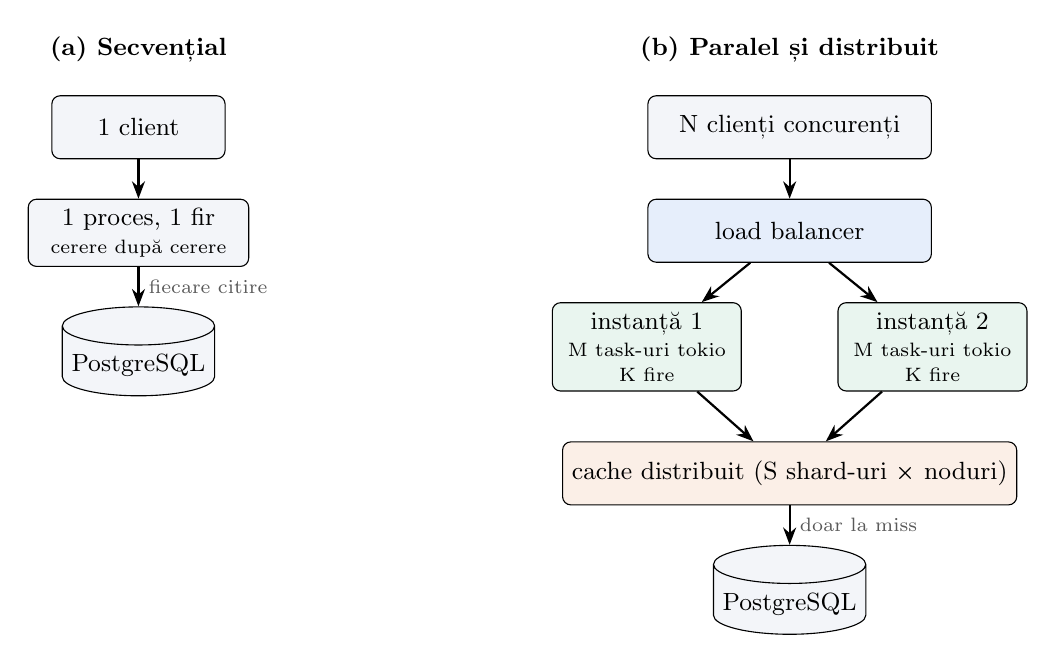
\begin{tikzpicture}[node distance=5mm and 7mm]
  \node[font=\small\bfseries] (t1) {(a) Secvențial};
  \node[comp, below=3mm of t1] (c1) {1 client};
  \node[comp, below=of c1, minimum width=28mm] (p1) {1 proces, 1 fir\\[-1pt]\scriptsize cerere după cerere};
  \node[store, below=of p1] (d1) {PostgreSQL};
  \draw[arr] (c1) -- (p1); \draw[arr] (p1) -- node[note, right] {fiecare citire} (d1);

  \node[font=\small\bfseries, right=50mm of t1] (t2) {(b) Paralel și distribuit};
  \node[comp, below=3mm of t2, minimum width=36mm] (c2) {N clienți concurenți};
  \node[comp, below=of c2, minimum width=36mm, fill=c1!12] (lb) {load balancer};
  \node[comp, below left=5mm and -12mm of lb, minimum width=24mm, fill=c3!10] (i1) {instanță 1\\[-1pt]\scriptsize M task-uri tokio\\[-2pt]\scriptsize K fire};
  \node[comp, below right=5mm and -12mm of lb, minimum width=24mm, fill=c3!10] (i2) {instanță 2\\[-1pt]\scriptsize M task-uri tokio\\[-2pt]\scriptsize K fire};
  \node[comp, below=12mm of $(i1)!0.5!(i2)$, minimum width=42mm, fill=c2!12] (cc) {cache distribuit (S shard-uri × noduri)};
  \node[store, below=of cc] (d2) {PostgreSQL};
  \draw[arr] (c2) -- (lb); \draw[arr] (lb) -- (i1); \draw[arr] (lb) -- (i2);
  \draw[arr] (i1) -- (cc); \draw[arr] (i2) -- (cc);
  \draw[arr] (cc) -- node[note, right] {doar la miss} (d2);
\end{tikzpicture}
}
  \caption{Arhitectura secvențială (a) față de arhitectura paralelă și distribuită (b).}
  \label{fig:seqpar}
\end{figure}

Arhitectura propusă (\cref{fig:seqpar}b) introduce paralelism pe mai multe niveluri:

\begin{table}[H]
\centering\small
\begin{tabularx}{\linewidth}{lXl}
\toprule
Nivel & Mecanism & Tip \\
\midrule
Cereri & runtime asincron tokio: mii de task-uri multiplexate pe un pool de fire (work-stealing) & concurență + paralelism \\
Structura de date & \texttt{memtable}: $S$ shard-uri independente, fiecare cu propriul mutex & paralelism pe date \\
Instanțe & 2 instanțe web identice, fără stare, în spatele nginx (\texttt{least\_conn}) & scalare orizontală \\
Cache distribuit & $n$ noduri, chei partiționate prin consistent hashing & partiționare (sharding) \\
Invalidare & difuzare paralelă a invalidărilor pe tag (\texttt{JoinSet}) și \texttt{NOTIFY} & comunicare distribuită \\
Scrieri & write-behind: 4 workeri asincroni, partiționați după cheie, grupează scrierile în loturi & pipeline producător–consumator \\
\bottomrule
\end{tabularx}
\caption{Nivelurile de paralelism și distribuire.}
\end{table}

\subsection{Descompunerea problemei}

Cererile HTTP sunt independente (\emph{embarrassingly parallel}); singurele puncte de sincronizare sunt
structurile partajate: cache-ul și baza de date. Sharding-ul elimină sincronizarea globală în cache:
două chei din shard-uri diferite pot fi accesate simultan fără coordonare. Pentru cache-ul distribuit,
partiționarea prin consistent hashing face ca fiecare cheie să aibă un singur proprietar, deci nu este
nevoie de protocoale de consens; singura operație care atinge toate nodurile este invalidarea pe tag.

\subsection{Comunicare și sincronizare}

\begin{itemize}
  \item instanță ↔ nod de cache: protocol text binary-safe peste TCP, conexiuni persistente din pool,
        suport pentru \emph{pipelining};
  \item instanță ↔ PostgreSQL: pool de conexiuni (sqlx); notificări asincrone prin \texttt{LISTEN};
  \item în proces: \texttt{Mutex} per shard, \texttt{RwLock} pentru configurația curentă (înlocuită
        atomic prin \texttt{Arc}), canal \texttt{mpsc} mărginit pentru write-behind (\emph{backpressure}),
        \texttt{OnceCell} per cheie pentru single-flight.
\end{itemize}

\subsection{Compromisuri}

Distribuirea aduce costuri noi: o ședere în rețea per acces (≈100–300 µs față de ≈1 µs pentru L1),
problema coerenței între instanțe și complexitate operațională. De aceea sistemul oferă și varianta pe
două niveluri (L1 local cu TTL scurt + L2 distribuit), care combină latența cache-ului local cu
capacitatea agregată a clusterului.

\chapter{Arhitectura sistemului}
\label{ch:arhitectura}

\section{Vedere de ansamblu}

\Cref{fig:arch} prezintă arhitectura de implementare. Toate componentele rulează ca containere
Docker orchestrate cu Docker Compose, într-o rețea virtuală comună.

\begin{figure}[H]
  \centering
  \resizebox{\linewidth}{!}{% Arhitectura distribuită (docker compose).
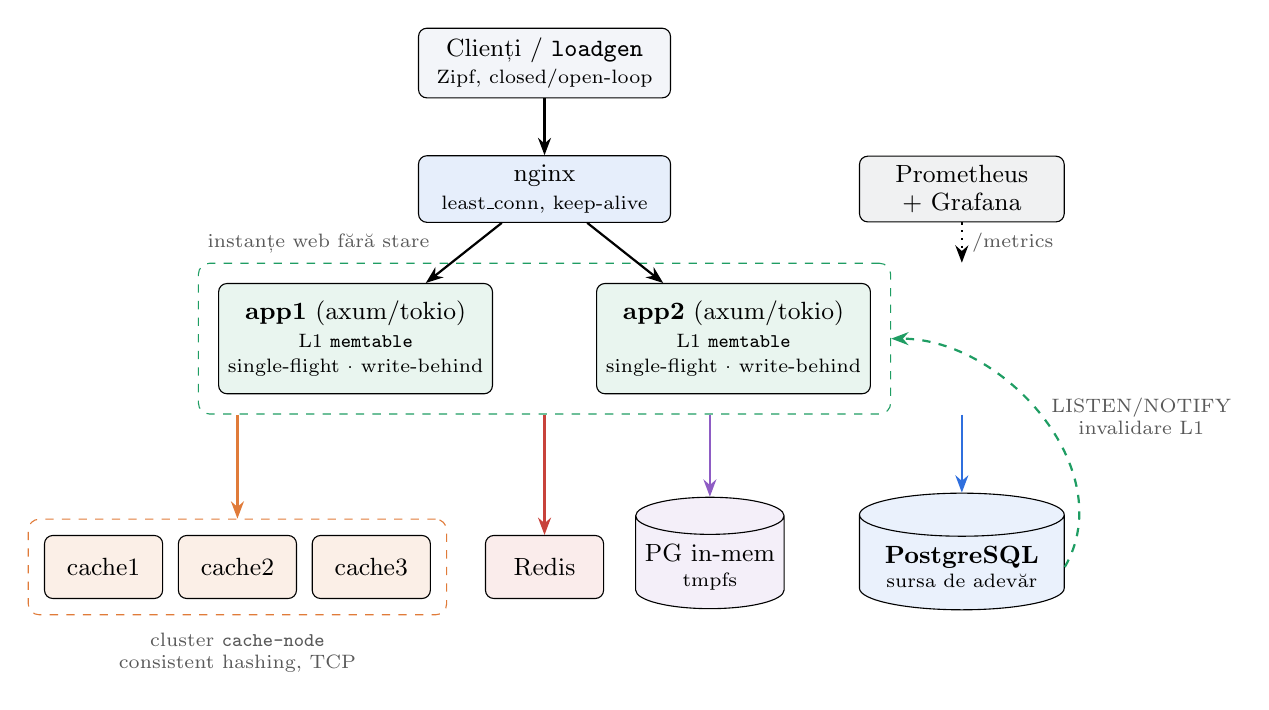
\begin{tikzpicture}
  \node[comp, minimum width=32mm] (cli) at (0,0) {Clienți / \texttt{loadgen}\\[-1pt]\scriptsize Zipf, closed/open-loop};
  \node[comp, minimum width=32mm, fill=c1!12] (lb) at (0,-1.6) {nginx\\[-1pt]\scriptsize least\_conn, keep-alive};
  \node[comp, minimum width=34mm, minimum height=14mm, fill=c3!10] (a1) at (-2.4,-3.5) {\textbf{app1} (axum/tokio)\\[-1pt]\scriptsize L1 \texttt{memtable}\\[-2pt]\scriptsize single-flight · write-behind};
  \node[comp, minimum width=34mm, minimum height=14mm, fill=c3!10] (a2) at (2.4,-3.5) {\textbf{app2} (axum/tokio)\\[-1pt]\scriptsize L1 \texttt{memtable}\\[-2pt]\scriptsize single-flight · write-behind};
  \begin{scope}[on background layer]
    \node[draw=c3, dashed, rounded corners, fit=(a1)(a2), inner sep=2.5mm] (apps) {};
  \end{scope}
  \node[note, anchor=south west] at (apps.north west) {instanțe web fără stare};
  \draw[arr] (cli) -- (lb);
  \draw[arr] (lb) -- (a1); \draw[arr] (lb) -- (a2);

  % Backend-uri.
  \node[comp, minimum width=15mm, fill=c2!12] (n1) at (-5.6,-6.4) {cache1};
  \node[comp, minimum width=15mm, fill=c2!12] (n2) at (-3.9,-6.4) {cache2};
  \node[comp, minimum width=15mm, fill=c2!12] (n3) at (-2.2,-6.4) {cache3};
  \begin{scope}[on background layer]
    \node[draw=c2, dashed, rounded corners, fit=(n1)(n3), inner sep=2mm] (ring) {};
  \end{scope}
  \node[note, below=1mm of ring] {cluster \texttt{cache-node}\\consistent hashing, TCP};
  \node[comp, minimum width=15mm, fill=c5!10] (rd) at (0,-6.4) {Redis};
  \node[store, fill=c4!10] (pm) at (2.1,-6.4) {PG in-mem\\[-2pt]\scriptsize tmpfs};
  \node[store, minimum width=26mm, minimum height=13mm, fill=c1!10] (db) at (5.3,-6.4) {\textbf{PostgreSQL}\\[-2pt]\scriptsize sursa de adevăr};

  \foreach \t/\c in {ring/c2, rd/c5, pm/c4, db/c1} {
    \draw[arr, \c] (apps.south -| \t.north) -- (\t.north);
  }
  \draw[arr, dashed, c3] (db.east) to[out=60,in=0] node[note, right, pos=0.5] {LISTEN/NOTIFY\\invalidare L1} (apps.east);

  \node[comp, minimum width=26mm, fill=c6!10] (obs) at (5.3,-1.6) {Prometheus\\[-1pt]+ Grafana};
  \draw[arr, dotted] (obs.south) -- node[note, right] {/metrics} (obs.south |- apps.north);
\end{tikzpicture}
}
  \caption{Arhitectura distribuită a sistemului.}
  \label{fig:arch}
\end{figure}

\begin{table}[H]
\centering\small
\begin{tabularx}{\linewidth}{lcX}
\toprule
Componentă & Instanțe & Rol \\
\midrule
\texttt{nginx} & 1 & load balancer HTTP (\texttt{least\_conn}, conexiuni keep-alive către backend) \\
\texttt{webapp} & 2 & API REST (axum); cache L1 \texttt{memtable}; single-flight; write-behind; metrici \\
\texttt{cache-node} & 3 & server TCP peste \texttt{memtable}; partiționare prin consistent hashing \\
PostgreSQL & 1 & baza relațională — sursa de adevăr; trigger \texttt{NOTIFY} \\
PostgreSQL in-memory & 1 & date pe \texttt{tmpfs}, \texttt{fsync=off}; tabela \texttt{UNLOGGED cache\_kv} \\
Redis & 1 & cache de referință (\emph{baseline} industrial), fără persistență \\
Prometheus, Grafana & 1+1 & colectare metrici (2 s) și dashboard provizionat automat \\
\texttt{loadgen} & la cerere & generator de încărcare și benchmark-uri offline \\
\bottomrule
\end{tabularx}
\caption{Componentele sistemului.}
\end{table}

\section{Organizarea codului}

Proiectul este un \emph{workspace} Cargo cu patru crate-uri, cu dependențe aciclice:

\begin{center}
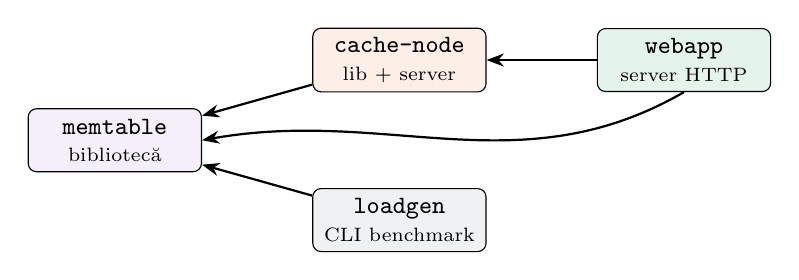
\begin{tikzpicture}[node distance=6mm and 12mm]
  \node[comp, fill=c4!10] (m) {\texttt{memtable}\\[-1pt]\scriptsize bibliotecă};
  \node[comp, fill=c2!12, above right=2mm and 14mm of m] (c) {\texttt{cache-node}\\[-1pt]\scriptsize lib + server};
  \node[comp, fill=c3!12, right=14mm of c] (w) {\texttt{webapp}\\[-1pt]\scriptsize server HTTP};
  \node[comp, fill=c6!10, below right=2mm and 14mm of m] (l) {\texttt{loadgen}\\[-1pt]\scriptsize CLI benchmark};
  \draw[arr] (c) -- (m); \draw[arr] (w) -- (c); \draw[arr] (w.south) to[out=-150,in=10] (m.east); \draw[arr] (l) -- (m);
\end{tikzpicture}
\end{center}

\begin{itemize}
  \item \texttt{memtable} — motorul de tabele in-memory, fără dependențe de rețea; reutilizat de nodurile
        de cache, de aplicație (L1) și de benchmark-uri.
  \item \texttt{cache-node} — protocolul, serverul TCP, clientul cu pool de conexiuni, inelul de
        consistent hashing și clientul de cluster.
  \item \texttt{webapp} — aplicația web: rute, OpenAPI, backend-uri de cache, strategii, metrici, UI.
  \item \texttt{loadgen} — încărcare HTTP, simulare de politici, scalabilitatea motorului.
\end{itemize}

\section{Motorul de tabele in-memory}

\begin{figure}[H]
  \centering
  \resizebox{0.92\linewidth}{!}{% Structura internă a unei tabele memtable.
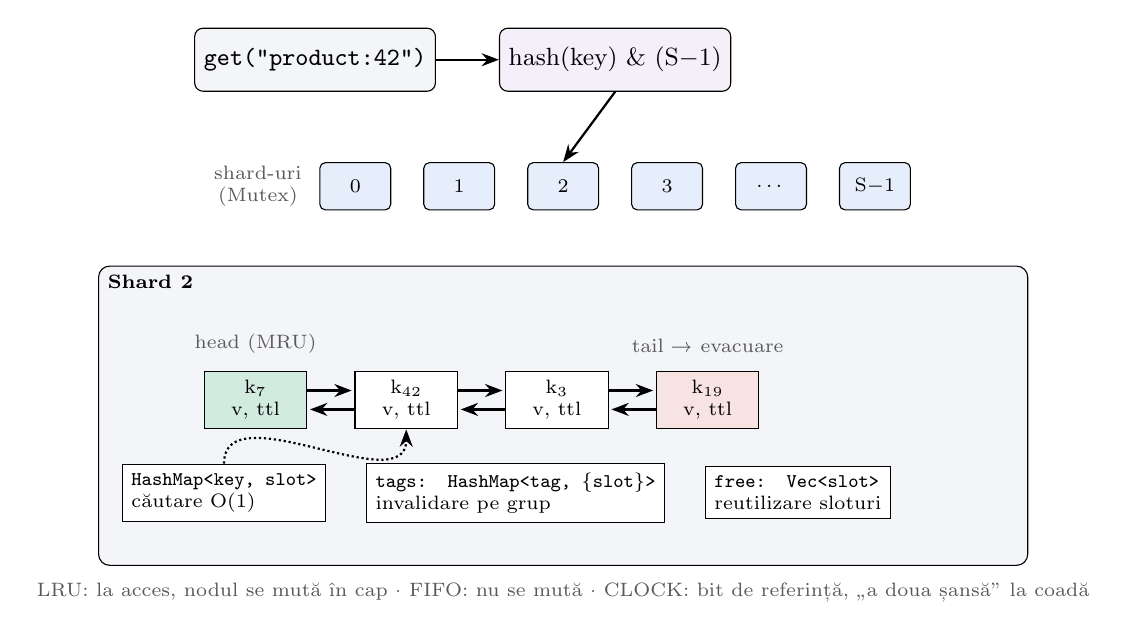
\begin{tikzpicture}[
  slot/.style={draw, minimum width=13mm, minimum height=7mm, font=\scriptsize, fill=white, align=center},
  sh/.style={draw, rounded corners=2pt, minimum width=9mm, minimum height=6mm, font=\scriptsize, fill=c1!12}]
  \node[comp, minimum width=26mm] (k) {\texttt{get("product:42")}};
  \node[comp, right=8mm of k, minimum width=24mm, fill=c4!10] (h) {hash(key) \& (S$-$1)};
  \draw[arr] (k) -- (h);
  \foreach \i in {0,...,5} { \node[sh] (s\i) at ($(h.south)+(-3.3+1.32*\i,-1.2)$) {\ifnum\i=5 S$-$1\else\ifnum\i=4 …\else\i\fi\fi}; }
  \draw[arr] (h.south) -- (s2.north);
  \node[note, left=1mm of s0] {shard-uri\\(Mutex)};

  % Detaliul unui shard.
  \node[draw, rounded corners, fill=boxbg, minimum width=118mm, minimum height=38mm, below=7mm of s2.south, anchor=north] (box) {};
  \node[font=\scriptsize\bfseries, anchor=north west] at (box.north west) {Shard 2};
  \node[slot, fill=c3!20] (e1) at ($(box.west)+(20mm,2mm)$) {k$_7$\\v, ttl};
  \node[slot, right=6mm of e1] (e2) {k$_{42}$\\v, ttl};
  \node[slot, right=6mm of e2] (e3) {k$_3$\\v, ttl};
  \node[slot, right=6mm of e3, fill=c5!15] (e4) {k$_{19}$\\v, ttl};
  \foreach \a/\b in {e1/e2,e2/e3,e3/e4} {
    \draw[arr, shorten >=1pt] ([yshift=1.2mm]\a.east) -- ([yshift=1.2mm]\b.west);
    \draw[arr, shorten >=1pt] ([yshift=-1.2mm]\b.west) -- ([yshift=-1.2mm]\a.east);
  }
  \node[note, above=1mm of e1] {head (MRU)};
  \node[note, above=1mm of e4] {tail → evacuare};
  \node[draw, font=\scriptsize, align=left, fill=white, anchor=north west] (map) at ($(box.south west)+(3mm,13mm)$) {\texttt{HashMap<key, slot>}\\ căutare O(1)};
  \node[draw, font=\scriptsize, align=left, fill=white, right=5mm of map] (tags) {\texttt{tags: HashMap<tag, \{slot\}>}\\ invalidare pe grup};
  \node[draw, font=\scriptsize, align=left, fill=white, right=5mm of tags] (free) {\texttt{free: Vec<slot>}\\ reutilizare sloturi};
  \draw[arr, densely dotted] (map.north) to[out=90,in=-90] (e2.south);
  \node[note, below=1mm of box] {LRU: la acces, nodul se mută în cap · FIFO: nu se mută · CLOCK: bit de referință, „a doua șansă" la coadă};
\end{tikzpicture}
}
  \caption{Structura unei tabele \texttt{memtable}: shard-uri independente, fiecare cu un hash map,
           o listă dublu înlănțuită intrusivă peste un slab și un index de tag-uri.}
  \label{fig:memtable}
\end{figure}

O tabelă (\cref{fig:memtable}) este împărțită în $S$ shard-uri ($S$ putere a lui 2). Cheia este
direcționată către shard prin $\text{hash}(k) \mathbin{\&} (S-1)$, iar fiecare shard este protejat de
propriul mutex. În interiorul shard-ului:

\begin{itemize}
  \item intrările sunt stocate într-un \emph{slab} (\texttt{Vec<Slot>}); legăturile listei sunt indici
        \texttt{u32}, nu pointeri — fără \texttt{unsafe}, cu localitate bună în cache-ul procesorului;
  \item un \texttt{HashMap<cheie, index>} oferă căutare O(1);
  \item lista dublu înlănțuită ordonează intrările pentru evacuare: capul este cea mai recentă, coada este
        candidatul; toate operațiile (acces, inserare, ștergere, evacuare) sunt O(1);
  \item indexul de tag-uri \texttt{HashMap<tag, \{index\}>} permite invalidarea unui grup de chei (de
        exemplu toate clasamentele unei categorii) fără a parcurge tabela;
  \item sloturile eliberate sunt reținute într-o listă liberă și refolosite (fără realocări).
\end{itemize}

Valorile sunt \texttt{bytes::Bytes} — buffere imutabile cu numărare de referințe, deci un hit nu copiază
datele: același buffer ajunge direct în corpul răspunsului HTTP.

\section{Cache-ul distribuit}

\begin{figure}[H]
  \centering
  \begin{subfigure}{0.42\linewidth}\centering
    \resizebox{\linewidth}{!}{% Inelul de consistent hashing cu noduri virtuale.
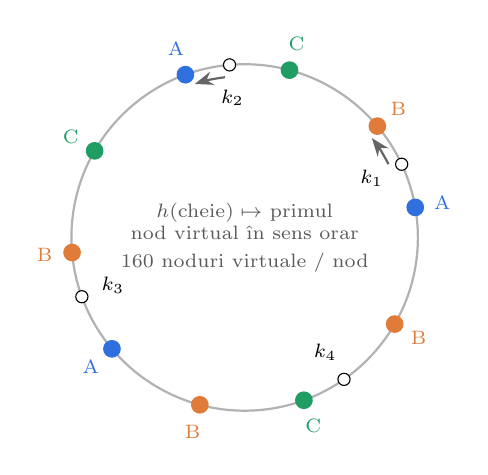
\begin{tikzpicture}
  \def\R{2.2}
  \draw[thick, gray!60] (0,0) circle (\R);
  \foreach \ang/\col/\lab in {10/c1/A,40/c2/B,75/c3/C,110/c1/A,150/c3/C,185/c2/B,220/c1/A,255/c2/B,290/c3/C,330/c2/B} {
    \fill[\col] (\ang:\R) circle (3.2pt);
    \node[font=\scriptsize, text=\col] at (\ang:\R+0.35) {\lab};
  }
  \foreach \ang/\k in {25/k_1,95/k_2,200/k_3,305/k_4} {
    \draw[fill=white, draw=black] (\ang:\R) circle (2.2pt);
    \node[font=\scriptsize] at (\ang:\R-0.42) {$\k$};
  }
  \draw[-{Stealth}, thick, black!60] (27:\R-0.15) arc (27:38:\R-0.15);
  \draw[-{Stealth}, thick, black!60] (97:\R-0.15) arc (97:108:\R-0.15);
  \node[note, align=center] at (0,0) {$h(\text{cheie}) \mapsto$ primul\\nod virtual în sens orar\\[2pt] 160 noduri virtuale / nod};
\end{tikzpicture}
}
    \caption{Inelul de consistent hashing.}
    \label{fig:ring}
  \end{subfigure}\hfill
  \begin{subfigure}{0.54\linewidth}\centering\small
    \begin{tabular}{@{}ll@{}}
      \toprule
      Comandă & Răspuns \\
      \midrule
      \texttt{GET k} & \texttt{\$len\textbackslash n bytes} / \texttt{\$-1} \\
      \texttt{SET k ttl len [tags]} & \texttt{+OK} \\
      \texttt{DEL k} & \texttt{:1} / \texttt{:0} \\
      \texttt{TAG t} & \texttt{:n} \\
      \texttt{STATS} & \texttt{\$len\textbackslash n json} \\
      \texttt{CONFIG cap pol shards} & \texttt{+OK} \\
      \bottomrule
    \end{tabular}
    \caption{Protocolul nodului (extras).}
  \end{subfigure}
  \caption{Partiționarea și protocolul cache-ului distribuit.}
\end{figure}

Nodurile nu comunică între ele: partiționarea este realizată în client. Fiecare nod fizic este plasat
de 160 de ori pe un inel de $2^{64}$ poziții, folosind o funcție de dispersie stabilă (FNV-1a urmată de
un finalizator \emph{splitmix64}). Căutarea nodului responsabil se face prin căutare binară în vectorul
sortat al punctelor, în $O(\log(160n))$. Testele unitare verifică echilibrul (fiecare din 3 noduri
primește între 27\% și 40\% din chei) și faptul că adăugarea unui al patrulea nod mută
$\approx 25\%$ din chei.

Protocolul este textual pentru antete și binar pentru valori (prefixate cu lungimea), deci poate
transporta orice conținut. Serverul trimite răspunsurile (\emph{flush}) doar când bufferul de intrare
s-a golit, ceea ce permite \emph{pipelining}: un client poate trimite mai multe comenzi fără să aștepte
fiecare răspuns.

\section{Fluxul unei cereri de citire}

\begin{figure}[H]
  \centering
  \resizebox{0.95\linewidth}{!}{% Diagrama de secvență: citire cache-aside cu single-flight.
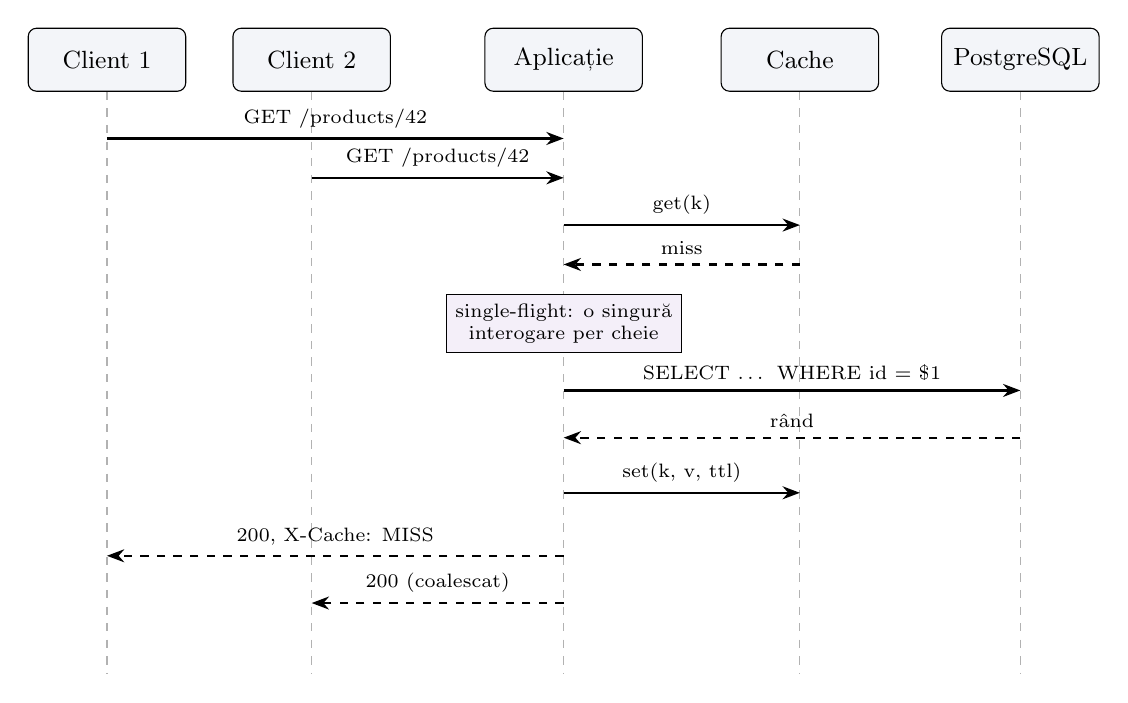
\begin{tikzpicture}[font=\small]
  \foreach \x/\n/\t in {0/c1/Client 1,2.6/c2/Client 2,5.8/app/Aplicație,8.8/cache/Cache,11.6/db/PostgreSQL} {
    \node[comp, minimum width=20mm] (\n) at (\x,0) {\t};
    \draw[gray!60, dashed] (\n.south) -- ++(0,-7.4);
  }
  \newcommand{\msg}[5][]{\draw[arr,#1] (#2,#4) -- node[above, font=\scriptsize]{#5} (#3,#4);}
  \msg{0}{5.8}{-1.0}{GET /products/42}
  \msg{2.6}{5.8}{-1.5}{GET /products/42}
  \msg{5.8}{8.8}{-2.1}{get(k)}
  \msg[dashed]{8.8}{5.8}{-2.6}{miss}
  \node[draw, fill=c4!10, font=\scriptsize, align=center] at (5.8,-3.35) {single-flight: o singură\\interogare per cheie};
  \msg{5.8}{11.6}{-4.2}{SELECT … WHERE id = \$1}
  \msg[dashed]{11.6}{5.8}{-4.8}{rând}
  \msg{5.8}{8.8}{-5.5}{set(k, v, ttl)}
  \msg[dashed]{5.8}{0}{-6.3}{200, X-Cache: MISS}
  \msg[dashed]{5.8}{2.6}{-6.9}{200 (coalescat)}
\end{tikzpicture}
}
  \caption{Citire cache-aside cu single-flight: două cereri concurente pentru aceeași cheie produc o
           singură interogare SQL.}
  \label{fig:readpath}
\end{figure}

La un miss, aplicația nu interoghează imediat baza de date: verifică într-o tabelă de „zboruri în
curs" (\texttt{HashMap<cheie, Arc<OnceCell>>}) dacă o altă cerere încarcă deja aceeași cheie. Dacă da,
așteaptă rezultatul acesteia (\cref{fig:readpath}). Mecanismul elimină \emph{cache stampede} la pornire
sau după invalidarea unei chei fierbinți (experimentul E7).

\section{Strategiile de scriere}

\begin{figure}[H]
  \centering
  \resizebox{\linewidth}{!}{% Cele trei strategii de scriere.
\begin{tikzpicture}[font=\small, node distance=4mm]
  \foreach \col/\x/\title/\a/\b/\c in {
      c1/0/Invalidate (cache-aside)/1. UPDATE în DB/2. DEL cheie din cache/3. următoarea citire: miss → DB,
      c3/5.2/Write-through/1. UPDATE în DB/2. SET valoarea nouă în cache/3. citirile rămân hit,
      c2/10.4/Write-behind/1. SET în cache; răspuns 202/2. coadă → lot (≤1024)/3. un UPDATE … unnest()} {
    \node[draw=\col, very thick, rounded corners, minimum width=48mm, minimum height=27mm, fill=\col!6] (b) at (\x,0) {};
    \node[font=\small\bfseries, text=\col, anchor=north] at (b.north) {\title};
    \node[font=\scriptsize, align=left, anchor=north west] at ($(b.north west)+(2mm,-7mm)$) {\a\\[2pt]\b\\[2pt]\c};
  }
  \node[note, text width=46mm] at (0,-2.0) {+ simplu, corect\\− miss după fiecare scriere};
  \node[note, text width=46mm] at (5.2,-2.0) {+ hit ratio păstrat\\− latență de scriere mai mare};
  \node[note, text width=46mm] at (10.4,-2.0) {+ scrieri rapide, grupate\\− consistență eventuală, risc la crash};
\end{tikzpicture}
}
  \caption{Strategiile de scriere implementate.}
  \label{fig:writes}
\end{figure}

Pentru write-behind (\cref{fig:writes}, dreapta), modificările sunt distribuite pe 4 benzi paralele după
\texttt{id mod 4}. Toate modificările unui produs trec prin aceeași bandă, deci ordinea lor se păstrează.
Fiecare bandă este un canal mărginit (25.000 de elemente), care oferă \emph{backpressure}: dacă baza de
date nu ține pasul, cererile de scriere așteaptă în loc să acumuleze o coadă nelimitată. Workerul fiecărei
benzi preia până la 1.024 de modificări deodată, le combină per produs (ultima scriere câștigă, pe câmp) și
le aplică printr-un singur \texttt{UPDATE \ldots{} FROM unnest(\ldots)}. După flush, invalidarea
clasamentelor categoriilor afectate rulează concurent, într-un task separat.
La oprirea aplicației (SIGTERM), canalul este închis și golit complet înainte de terminarea procesului.

\section{Coerența cache-urilor locale}

Fiecare instanță are propriul L1. Un trigger \texttt{AFTER UPDATE} pe tabela \texttt{products} execută
\texttt{pg\_notify} pe canalul \texttt{cache\_invalidation}, cu mesajul \texttt{id:categorie}; fiecare instanță ține o conexiune dedicată
cu \texttt{LISTEN} și, la primirea notificării, șterge cheia produsului și tag-ul categoriei din L1.
Avantajul major: și modificările făcute direct în baza de date (scripturi, alte aplicații) invalidează
cache-ul. Pentru că \texttt{NOTIFY} serializează commit-urile (\cref{sec:optimizari}), aplicația îl
suprimă (\texttt{app.notify = off}) când backend-ul activ nu are nivel local.

\section{Reziliență}

\begin{itemize}
  \item \textbf{Degradare grațioasă}: orice eroare a backend-ului de cache este contorizată și cererea
        continuă direct pe baza de date.
  \item \textbf{Conexiuni}: clientul de nod reîncearcă o dată cu o conexiune nouă dacă o conexiune din pool
        s-a închis (nod repornit); conectarea la baze de date se reîncearcă la pornire.
  \item \textbf{Ascultătorul NOTIFY} se reconectează automat.
  \item \textbf{Write-behind}: reîncercări cu \emph{backoff} exponențial (8 încercări) și golirea cozii la oprire.
\end{itemize}

\chapter{Implementare}
\label{ch:implementare}

\section{Motorul \texttt{memtable}}

Operația de citire dintr-un shard ilustrează politicile de evacuare: expirarea TTL este verificată leneș
la acces, iar efectul unui hit depinde de politică.

\begin{code}{Citirea dintr-un shard (\texttt{crates/memtable/src/shard.rs}).}
pub(crate) fn get(&mut self, key: &str, now: Instant) -> Lookup {
    let Some(&i) = self.map.get(key) else { return Lookup::Miss };
    if self.entry(i).expires_at.is_some_and(|e| e <= now) {
        self.remove(i);              // expirare leneșă
        return Lookup::Expired;
    }
    self.touch(i);                   // LRU: mută în cap; CLOCK: bit = 1; FIFO: nimic
    Lookup::Hit(self.entry(i).value.clone())   // Bytes: clonare O(1), fără copiere
}
\end{code}

Evacuarea CLOCK parcurge coada: intrările cu bitul de referință setat primesc a doua șansă. Bucla se
termină după cel mult o trecere completă, deoarece fiecare intrare vizitată își pierde bitul.

\begin{code}{Evacuarea unei intrări.}
fn evict_one(&mut self) -> bool {
    loop {
        let t = self.tail;
        if t == NIL { return false; }
        if self.policy == Policy::Clock && self.entry(t).referenced {
            self.entry_mut(t).referenced = false;   // a doua șansă
            self.unlink(t);
            self.push_front(t);
            continue;
        }
        self.remove(t);
        return true;
    }
}
\end{code}

Statisticile sunt contoare atomice (\texttt{AtomicU64} cu ordonare \texttt{Relaxed}), actualizate în
afara secțiunii critice.

\section{Nodul de cache și clientul}

Serverul folosește un task tokio per conexiune. Bucla de tratare citește o linie de antet, apoi exact
\texttt{len} octeți de payload, și scrie răspunsul într-un \texttt{BufWriter}; flush-ul se face doar
când nu mai există comenzi în buffer. Erorile de protocol sunt raportate clientului fără a închide
conexiunea; erorile de I/O închid conexiunea. Un janitor elimină periodic intrările expirate.

Clientul păstrează un pool de conexiuni (\texttt{Mutex<Vec<BufStream<TcpStream>>>}); mutex-ul este
ținut doar pentru \texttt{pop}/\texttt{push}, niciodată în timpul unui \texttt{await}. Cheile și tag-urile
sunt validate la granița de încredere (fără spații sau virgule), iar valorile sunt limitate la 16 MiB pe
server.

\section{Aplicația web}

\subsection{Backend-uri interschimbabile}

Backend-urile sunt modelate ca \texttt{enum}, cu \emph{dispatch} static:

\begin{code}{Backend-urile de cache (\texttt{crates/webapp/src/cache.rs}).}
pub enum Backend {
    None,
    Local(Arc<Table>),                          // L1 în proces
    Cluster(ClusterClient),                     // noduri cache-node
    Redis(RedisConn),
    PgMem(PgPool),                              // tabelă UNLOGGED pe tmpfs
    Tiered { l1: Arc<Table>, l2: ClusterClient }, // near-cache
}
\end{code}

Configurația activă (\texttt{Runtime}: backend + parametri) este ținută într-un
\texttt{RwLock<Arc<Runtime>>}. Fiecare cerere clonează doar \texttt{Arc}-ul (o incrementare atomică), iar
schimbarea modului înlocuiește atomic pointerul — cererile în curs își termină execuția pe vechea
configurație.

\subsection{Single-flight}

\begin{code}{Single-flight cu \texttt{OnceCell} (\texttt{state.rs}, simplificat).}
let (cell, leader) = {
    let mut map = self.inflight.lock();
    match map.get(key) {
        Some(c) => (Arc::clone(c), false),
        None => { let c = Arc::default(); map.insert(key.into(), Arc::clone(&c)); (c, true) }
    }
};
let res = cell.get_or_init(move || async move { fetch.await }).await.clone();
// Oricine termină curăță intrarea (leader-ul poate fi anulat de deconectarea clientului).
let mut map = self.inflight.lock();
if map.get(key).is_some_and(|c| Arc::ptr_eq(c, &cell)) { map.remove(key); }
\end{code}

Un detaliu important: dacă cererea „lider" este anulată (clientul închide conexiunea), \texttt{OnceCell}
permite altei cereri să preia inițializarea, iar curățarea intrării este făcută de oricine termină —
altfel cheia ar rămâne blocată pe un rezultat vechi.

\subsection{API, documentație și interfață}

Rutele sunt definite cu axum 0.8; documentația OpenAPI 3 este generată din cod cu \texttt{utoipa}
(adnotări \texttt{\#[utoipa::path]} pe handlere și \texttt{ToSchema} pe tipuri) și servită prin Swagger UI
la \texttt{/swagger-ui}. Răspunsurile includ antetul \texttt{X-Cache}. Interfața web (\texttt{/}) este o
pagină statică inclusă în binar care permite schimbarea modului pe toate instanțele, afișează live rata de
hit și operațiile pe secundă (Chart.js), conține un generator de trafic Zipf rulat în browser și un
\emph{playground} pentru API.

\subsection{Observabilitate}

Un middleware măsoară latența fiecărei cereri într-o histogramă Prometheus etichetată cu ruta
(\texttt{MatchedPath}), metoda și codul de stare. Alte metrici: lookup-uri hit/miss, interogări DB pe tip,
erori ale backend-ului de cache și adâncimea cozii write-behind. Grafana este provizionată automat cu
sursa de date și un dashboard cu șase panouri.

\section{Optimizări}
\label{sec:optimizari}

Optimizările au fost ghidate de măsurători: o rulare scurtă (\texttt{scripts/profile.sh}) cu snapshot
de consum CPU per container, iterată după fiecare modificare.
\ifdefined\OptTable\OptTable\fi

\paragraph{1. Profilare: baza de date era gâtul de sticlă.} Înainte de optimizare, PostgreSQL consuma
$\approx$410\% din cele 500\% CPU disponibile, în timp ce fiecare instanță web consuma sub 20\%. Planul de
execuție al clasamentului unei categorii arăta un \emph{Parallel Seq Scan} pe 100.000 de produse și 500 de
accesări de heap pe \texttt{reviews} (7{,}6~ms).

\paragraph{2. Tuning PostgreSQL.} (a) \texttt{max\_parallel\_workers\_per\_gather = 0}: pentru un
volum OLTP mare, pornirea de workeri paraleli pentru fiecare interogare costă mai mult decât câștigă;
(b) indecși acoperitori \texttt{reviews(product\_id) INCLUDE (rating)} și
\texttt{products(category\_id) INCLUDE (id, name, price\_cents)} plus \texttt{VACUUM ANALYZE}, care
permit \emph{index-only scans}. Interogarea a scăzut de la 7{,}6~ms la 1{,}5~ms.

\paragraph{3. Calea fierbinte din aplicație.} Eliminarea \texttt{TraceLayer} (un span de tracing per
cerere), contoare Prometheus pre-rezolvate (fără căutarea etichetelor la fiecare cerere), evitarea
alocărilor în middleware, allocatorul \texttt{mimalloc} și reducerea pool-ului DB de la 32 la 16
conexiuni per instanță (mai puțină contenție în PostgreSQL).

\paragraph{4. \texttt{NOTIFY} condiționat.} Eșantionarea \texttt{pg\_stat\_activity} sub încărcare a arătat
majoritatea sesiunilor de scriere blocate în \texttt{Lock:object}: o tranzacție care execută
\texttt{NOTIFY} ține un lock global pe coada de notificări până după flush-ul WAL la commit, ceea ce
serializează toate scrierile și anulează \emph{group commit}. Trigger-ul notifică acum doar dacă sesiunea
nu a setat \texttt{app.notify = off}; aplicația setează valoarea (local tranzacției, prin
\texttt{set\_config(\ldots, true)} în aceeași instrucțiune \texttt{UPDATE}) când backend-ul nu are L1.
Scrierile externe continuă să fie notificate.

\paragraph{5. Agregate materializate.} Chiar și după pașii anteriori PostgreSQL rămânea la
$\approx$260\% CPU. Cauza: fiecare modificare de preț invalidează clasamentul categoriei; cu
$\approx$2.200 de scrieri/s distribuite pe 200 de categorii, aproape orice cerere de clasament era un miss
și recalcula un \texttt{JOIN} + \texttt{GROUP BY} de 1{,}5~ms. Media notelor și numărul de recenzii au
devenit coloane în \texttt{products} (\texttt{rating\_avg}, \texttt{review\_count}), întreținute incremental
de un trigger pe \texttt{reviews}, iar clasamentul folosește indexul
\texttt{(category\_id, rating\_avg DESC, review\_count DESC, id)}: interogarea durează acum
$\approx$0{,}09~ms (de 85 de ori mai puțin decât forma inițială). Citirea unui produs devine un lookup pe
cheia primară, iar scrierea întoarce rândul actualizat prin \texttt{RETURNING} (o interogare în loc de două).
Prețul nu este indexat și tabela are \texttt{fillfactor = 90}, deci actualizările de preț rămân
\emph{HOT} (nu modifică indecșii).

\paragraph{Rezultat.} Pe aceeași mașină, debitul cu cache local a crescut de la
\R{opt/baseline/rps} la \R{opt/mat-local/rps} cereri/s, iar p99 a scăzut de la \R{opt/baseline/p99}~ms la
\R{opt/mat-local/p99}~ms; varianta fără cache a crescut de la \R{opt/baseline-none/rps} la
\R{opt/mat-none/rps} cereri/s. Cu cache, consumul PostgreSQL a scăzut de la $\approx$410\% la
$\approx$60–100\% CPU; cei mai mari consumatori rămân nginx și generatorul de încărcare. Toate experimentele
din \cref{ch:evaluare} folosesc versiunea finală.

\section{Calitatea codului}

\begin{itemize}
  \item \textbf{Lint}: \texttt{clippy} cu grupurile \texttt{all} și \texttt{pedantic} la nivel de workspace,
        rulat cu \texttt{-D warnings}; \texttt{unsafe\_code = "forbid"}.
  \item \textbf{Formatare}: \texttt{rustfmt} (configurat în \texttt{rustfmt.toml}), \texttt{.editorconfig}.
  \item \textbf{Dependențe}: \texttt{cargo-deny} (licențe, vulnerabilități, surse) prin \texttt{deny.toml}.
  \item \textbf{Teste}: 19 teste unitare și de integrare (politici de evacuare, TTL, tag-uri,
        concurență, echilibrul inelului, roundtrip client–server, cluster, simulator) și un test end-to-end
        de coerență (\texttt{scripts/consistency.sh}) pentru toate cele 18 combinații backend × strategie.
  \item \textbf{CI}: GitHub Actions rulează formatarea, clippy, testele, \texttt{cargo-deny} și
        construirea imaginii Docker.
\end{itemize}

\chapter{Tehnologii utilizate}
\label{ch:tehnologii}

\begin{table}[H]
\centering\footnotesize
\renewcommand{\arraystretch}{1.05}
\begin{tabularx}{\linewidth}{@{}p{38mm}X@{}}
\toprule
Tehnologie & Utilizare și motivație \\
\midrule
\textbf{Rust} (ediția 2024) & limbaj de sistem cu siguranța memoriei garantată la compilare, fără
  garbage collector (latențe predictibile), cu abstracții de cost zero. Sistemul de tipuri previne
  \emph{data race}-urile: \texttt{Send}/\texttt{Sync} verifică la compilare ce poate fi partajat între fire. \\
\textbf{tokio} & runtime asincron cu planificator \emph{work-stealing} pe mai multe fire: mii de conexiuni
  concurente cu un număr mic de fire de sistem; primitive \texttt{mpsc}, \texttt{watch}, \texttt{OnceCell},
  \texttt{JoinSet}. \\
\textbf{axum} 0.8 & framework HTTP peste hyper/tower; extractori tipizați, middleware. \\
\textbf{sqlx} 0.8 & driver PostgreSQL asincron, pool de conexiuni, \emph{prepared statements} memorate per
  conexiune, \texttt{PgListener} pentru \texttt{LISTEN}. \\
\textbf{redis-rs} & client Redis cu \texttt{ConnectionManager} (conexiune multiplexată, reconectare). \\
\textbf{utoipa} + Swagger UI & specificație OpenAPI 3 generată din cod; documentație interactivă. \\
\textbf{prometheus} & metrici în format text expuse la \texttt{/metrics}. \\
\textbf{parking\_lot} & mutex-uri și RW-lock-uri mai mici și mai rapide decât cele din \texttt{std}. \\
\textbf{bytes} & buffere imutabile cu numărare de referințe — valori partajate fără copiere. \\
\textbf{mimalloc} & allocator global performant pentru alocări mici, concurente. \\
\textbf{hdrhistogram}, \textbf{rand\_distr} & histograme de latență cu precizie fixă; distribuția Zipf. \\
\textbf{reqwest} & client HTTP pentru generatorul de încărcare (pool keep-alive). \\
\textbf{clap} & interfețe CLI cu configurare din variabile de mediu. \\
\midrule
\textbf{PostgreSQL 17} & baza relațională (sursa de adevăr): tranzacții, indecși acoperitori, trigger-e
  PL/pgSQL, \texttt{LISTEN/NOTIFY}; a doua instanță cu tabelă \texttt{UNLOGGED} pe \texttt{tmpfs} ca
  „tabelă in-memory" relațională \cite{pg}. \\
\textbf{Redis 8} & cache in-memory de referință, \texttt{allkeys-lru}, fără persistență \cite{redis}. \\
\textbf{nginx} & load balancer HTTP cu conexiuni keep-alive către instanțe. \\
\textbf{Prometheus}, \textbf{Grafana} & monitorizare și vizualizare în timp real. \\
\textbf{Docker}, \textbf{Docker Compose} & împachetare (imagine multi-stage, utilizator neprivilegiat) și
  orchestrarea celor 12 containere; build-uri reproductibile (\texttt{Cargo.lock}, \texttt{--locked}). \\
\textbf{Chart.js} & grafice live în interfața web. \\
\textbf{GitHub Actions} & integrare continuă. \\
\textbf{\LaTeX} (LuaLaTeX, TikZ, pgfplots, Beamer) & documentația și prezentarea; graficele sunt
  generate direct din fișierele CSV ale experimentelor. \\
\bottomrule
\end{tabularx}
\caption{Tehnologiile utilizate.}
\end{table}

\section{Alternative considerate}

\begin{itemize}
  \item \textbf{\texttt{dyn Trait} vs. \texttt{enum}} pentru backend-uri: \texttt{enum} evită alocarea unui
        \texttt{Box<dyn Future>} per apel și dependența \texttt{async\_trait}; setul de backend-uri este închis.
  \item \textbf{HTTP vs. protocol TCP propriu} pentru nodurile de cache: un protocol minimal
        (în stilul RESP/memcached) are un cost de parsare mult mai mic decât HTTP și permite pipelining.
  \item \textbf{\texttt{RwLock} vs. \texttt{Mutex}} în shard-uri: o citire LRU modifică lista, deci are
        nevoie de acces exclusiv; un \texttt{RwLock} nu ar aduce beneficii și ar fi mai scump.
  \item \textbf{MySQL \texttt{MEMORY} engine} ca tabelă in-memory: are blocare la nivel de tabelă și nu
        suportă tipuri \texttt{BLOB/TEXT}; varianta PostgreSQL \texttt{UNLOGGED} pe \texttt{tmpfs} este
        echivalentă ca idee și păstrează aceeași tehnologie cu sursa de adevăr.
\end{itemize}

\chapter{Evaluarea performanțelor}
\label{ch:evaluare}

\section{Metodologie}

\paragraph{Mediu.} Toate componentele rulează pe aceeași mașină, într-un VM Docker Desktop cu
\textbf{5 vCPU} (Apple Silicon, arm64). Generatorul de încărcare, nginx, cele două instanțe, nodurile de
cache și bazele de date concurează pentru aceleași nuclee, deci rezultatele absolute sunt specifice
acestui mediu. Comparațiile între configurații sunt însă relevante, pentru că au fost obținute în
condiții identice.

\paragraph{Sarcina de lucru.} Generatorul \texttt{loadgen} rulează în rețeaua Docker și trimite cereri
prin nginx. Implicit folosește 64 de clienți \emph{closed-loop} (fiecare trimite cererea următoare
imediat după răspuns), 95\% citiri (din care 10\% clasamente de categorie), 5\% scrieri de preț și
popularitate Zipf cu $s = 0{,}99$ peste 100.000 de produse și 200 de categorii. Fiecare rulare are 5~s
de încălzire (nemăsurate) și 15~s de măsurare. Contoarele aplicației sunt resetate după încălzire.
Schimbarea modului golește cache-ul.

\paragraph{Metrici.} Debitul (cereri reușite/s), latențele p50/p95/p99 (histograme HDR, rezoluție 1~µs,
3 cifre semnificative), rata de hit (din contoarele aplicației, însumate pe instanțe), numărul de
interogări și tranzacții în baza de date. În E8, latența este măsurată de la momentul \emph{programat}
al cererii, ca să evităm \emph{coordinated omission} \cite{tene}.

\begin{table}[H]
\centering\small
\begin{tabularx}{\linewidth}{llX}
\toprule
Exp. & Variabilă & Întrebare \\
\midrule
E1 & backend (6) & Ce câștig aduce fiecare tip de cache față de baza de date? \\
E2 & exponent Zipf & Cum depinde rata de hit de asimetria accesărilor, cu memorie limitată? \\
E3 & proporția de scrieri × strategie & Ce costă coerența la scriere? \\
E4 & clienți concurenți (1–256) & Cum scalează sistemul cu concurența? (1 client = secvențial) \\
E5 & instanțe web (1–2) & Câștig din scalarea orizontală? \\
E6 & noduri de cache (1–3) & Crește rata de hit cu memoria agregată a clusterului? \\
E7 & single-flight on/off & Cât reduce protecția la stampede încărcarea bazei? \\
E8 & backend, debit fix & Cât CPU costă o cerere în fiecare arhitectură? \\
SIM & politică × capacitate & Cât de aproape de optim sunt LRU/FIFO/CLOCK? \\
ENG & fire × shard-uri & Cât de bine se paralelizează motorul \texttt{memtable}? \\
\bottomrule
\end{tabularx}
\caption{Experimentele realizate.}
\end{table}

\section{E1 — Comparația backend-urilor}

\begin{figure}[H]
  \centering% E1 — comparația backend-urilor.
\begin{tikzpicture}
\begin{groupplot}[group style={group size=2 by 1, horizontal sep=17mm},
    width=0.5\linewidth, height=55mm, ybar, xtick=data,
    symbolic x coords={none,local,cluster,tiered,redis,pgmem},
    x tick label style={rotate=35, anchor=east, font=\footnotesize}, enlarge x limits=0.1]
  \nextgroupplot[ylabel={cereri / s}, bar width=8pt, ymin=0,
      nodes near coords, nodes near coords style={font=\tiny, rotate=90, anchor=west},
      point meta={\thisrow{rps}/1000}, nodes near coords={\pgfmathprintnumber[fixed,precision=1]{\pgfplotspointmeta}k},
      kticks, ymax=88000,
      title={\small (a) debit}]
    \addplot[fill=c1!70, draw=c1] table[x=backend, y=rps, col sep=comma] {\datadir e1.csv};
  \nextgroupplot[ylabel={latență (ms)}, ymode=log, bar width=5pt, log origin=infty,
      legend style={at={(0.02,0.98)}, anchor=north west}, title={\small (b) latență}]
    \addplot[fill=c3!70, draw=c3] table[x=backend, y=p50, col sep=comma] {\datadir e1.csv};
    \addplot[fill=c2!70, draw=c2] table[x=backend, y=p95, col sep=comma] {\datadir e1.csv};
    \addplot[fill=c5!70, draw=c5] table[x=backend, y=p99, col sep=comma] {\datadir e1.csv};
    \legend{p50, p95, p99}
\end{groupplot}
\end{tikzpicture}

  \caption{Debitul și latența pentru cele șase backend-uri (64 de clienți, 95\% citiri, Zipf 0,99).}
  \label{fig:e1}
\end{figure}

\begin{table}[H]
\centering\small
\begin{tabular}{lrrrr}
\toprule
Backend & cereri/s & p50 (ms) & p99 (ms) & hit (\%) \\
\midrule
\texttt{none}    & \R{e1/none/rps}    & \R{e1/none/p50}    & \R{e1/none/p99}    & — \\
\texttt{local}   & \R{e1/local/rps}   & \R{e1/local/p50}   & \R{e1/local/p99}   & \R{e1/local/hit} \\
\texttt{cluster} & \R{e1/cluster/rps} & \R{e1/cluster/p50} & \R{e1/cluster/p99} & \R{e1/cluster/hit} \\
\texttt{tiered}  & \R{e1/tiered/rps}  & \R{e1/tiered/p50}  & \R{e1/tiered/p99}  & \R{e1/tiered/hit} \\
\texttt{redis}   & \R{e1/redis/rps}   & \R{e1/redis/p50}   & \R{e1/redis/p99}   & \R{e1/redis/hit} \\
\texttt{pgmem}   & \R{e1/pgmem/rps}   & \R{e1/pgmem/p50}   & \R{e1/pgmem/p99}   & \R{e1/pgmem/hit} \\
\bottomrule
\end{tabular}
\caption{Rezultatele E1.}
\label{tab:e1}
\end{table}

\paragraph{Interpretare.} Toate cache-urile in-memory reale depășesc baza de date. Cache-ul local
are cel mai mare debit (\R{e1/local/rps} cereri/s, de \R{e1/local/speedup}× față de \texttt{none}) și cea mai
mică latență mediană (\R{e1/local/p50}~ms), pentru că un hit nu părăsește procesul. Rata lui de hit
(\R{e1/local/hit}\%) este însă mai mică decât a cache-urilor partajate (\R{e1/cluster/hit}\% pentru cluster,
\R{e1/redis/hit}\% pentru Redis). Cauza: fiecare dintre cele două instanțe își încălzește separat propria copie,
iar notificările \texttt{NOTIFY} invalidează ambele copii la fiecare scriere. Clusterul propriu
(\R{e1/cluster/rps} cereri/s) este comparabil cu Redis (\R{e1/redis/rps}), deși folosește un protocol și un
motor scrise de la zero.

Varianta \texttt{tiered} (\R{e1/tiered/rps}) are rata de hit cea mai mare, dar debit mai mic decât clusterul
simplu. Având un nivel local, ea reactivează \texttt{NOTIFY}, care serializează commit-urile
(\cref{sec:optimizari}), și dublează scrierile în cache la fiecare miss. Câștigul nivelului L1 apare doar
când latența rețelei până la L2 e mare, ceea ce nu e cazul într-o rețea Docker locală.

Rezultatul cel mai instructiv este \texttt{pgmem}: tabela in-memory din PostgreSQL este \emph{mai lentă} decât
baza de date fără cache (\R{e1/pgmem/rps} față de \R{e1/none/rps} cereri/s), deși are rată de hit
\R{e1/pgmem/hit}\%. Un hit costă aici la fel de mult ca interogarea originală: aceeași parsare, aceeași
execuție SQL și același pool de conexiuni. După optimizările din \cref{sec:optimizari}, interogarea sursă
este un simplu lookup pe cheia primară, servit din \emph{shared buffers}. Un miss costă chiar trei operații
(citire cache, citire DB, \emph{upsert}). Concluzia: \textbf{o tabelă in-memory într-un SGBD nu este un cache
eficient pentru date pe care SGBD-ul le servește deja din memorie}. Valoarea ei apare doar când rezultatul
cache-uit este mult mai scump decât un lookup.


\section{E2 — Asimetria accesărilor}

\begin{figure}[H]
  \centering% E2 — asimetria Zipf (cache = 10% din chei, doar citiri).
\begin{tikzpicture}
\begin{groupplot}[group style={group size=2 by 1, horizontal sep=17mm},
    width=0.5\linewidth, height=55mm, xlabel={exponent Zipf $s$}, xtick={0.6,0.8,0.99,1.2}]
  \nextgroupplot[ylabel={rata de hit}, ymin=0, ymax=1, legend pos=south east, title={\small (a) rata de hit}]
    \addplot table[x=label, y=local_hit_ratio, col sep=comma] {\datadir e2.csv};
    \addplot table[x=label, y=cluster_hit_ratio, col sep=comma] {\datadir e2.csv};
    \addplot[c6, thick, dashed, mark=o] table[x=label, y=ideal, col sep=comma] {\datadir e2.csv};
    \legend{local, cluster, ideal IRM}
  \nextgroupplot[ylabel={cereri / s}, ymin=0, legend pos=north west, title={\small (b) debit},
      kticks]
    \addplot[c6, mark=o, thick] table[x=label, y=none_throughput_rps, col sep=comma] {\datadir e2.csv};
    \addplot table[x=label, y=local_throughput_rps, col sep=comma] {\datadir e2.csv};
    \addplot table[x=label, y=cluster_throughput_rps, col sep=comma] {\datadir e2.csv};
    \legend{none, local, cluster}
\end{groupplot}
\end{tikzpicture}

  \caption{Rata de hit și debitul în funcție de exponentul Zipf. Cache-ul are 10\% din chei, iar
           traficul conține doar citiri. Linia punctată este limita teoretică IRM (\cref{eq:ideal}).}
  \label{fig:e2}
\end{figure}

\paragraph{Interpretare.} Cu memoria limitată la 10\% din chei, rata de hit crește puternic cu asimetria:
de la \R{e2/local/0.6/hit_ratio}\% la $s=0{,}6$ la \R{e2/local/1.2/hit_ratio}\% la $s=1{,}2$. Valorile urmăresc
îndeaproape limita teoretică IRM (\cref{eq:ideal}): diferența de 2–8 puncte reprezintă costul unei politici
\emph{online} (LRU) față de cache-ul static optim. Cele două backend-uri au practic aceeași rată de hit, pentru
că au aceeași capacitate totală.

Debitul cache-ului local se dublează pe intervalul studiat (\R{e2/local/0.6/throughput_rps} $\rightarrow$
\R{e2/local/1.2/throughput_rps} cereri/s), în timp ce baza de date rămâne aproape constantă. La asimetrie mică
($s=0{,}6$), clusterul este însă \emph{mai lent} decât baza de date (\R{e2/cluster/0.6/throughput_rps} față de
\R{e2/none/0.6/throughput_rps}). Explicația vine din \cref{eq:amat}: un cache la distanță adaugă o ședere în
rețea fiecărei cereri, deci câștigă doar dacă $h > T_{\text{cache}}/T_{\text{DB}}$. Când interogarea sursă este
ieftină, pragul de rentabilitate este ridicat, iar cu doar \R{e2/cluster/0.6/hit_ratio}\% hit-uri el nu este atins.


\section{E3 — Strategii de scriere}

\begin{figure}[H]
  \centering% E3 — strategii de scriere.
\begin{tikzpicture}
\begin{groupplot}[group style={group size=2 by 1, horizontal sep=17mm},
    width=0.5\linewidth, height=55mm, xlabel={proporția de citiri}, xtick={0.5,0.8,0.95}]
  \nextgroupplot[ylabel={cereri / s}, ymin=0, legend pos=south east, title={\small (a) debit},
      kticks]
    \addplot table[x=label, y=invalidate_throughput_rps, col sep=comma] {\datadir e3.csv};
    \addplot table[x=label, y=write-through_throughput_rps, col sep=comma] {\datadir e3.csv};
    \addplot table[x=label, y=write-behind_throughput_rps, col sep=comma] {\datadir e3.csv};
    \legend{invalidate, write-through, write-behind}
  \nextgroupplot[ylabel={tranzacții DB / 1000 scrieri}, ymode=log, ymin=150, ymax=1300, ytick={200,300,500,1000}, log ticks with fixed point,
      title={\small (b) scrieri în DB}]
    \addplot table[x=label, y=invalidate_tx_per_1k, col sep=comma] {\datadir e3.csv};
    \addplot table[x=label, y=write-through_tx_per_1k, col sep=comma] {\datadir e3.csv};
    \addplot table[x=label, y=write-behind_tx_per_1k, col sep=comma] {\datadir e3.csv};
\end{groupplot}
\end{tikzpicture}

  \caption{Debitul și numărul de tranzacții în baza de date la 1.000 de scrieri, pentru cele trei
           strategii (backend \texttt{cluster}).}
  \label{fig:e3}
\end{figure}

\paragraph{Interpretare.} Diferențele apar la proporții mari de scrieri. La 50\% scrieri, invalidarea păstrează
doar \R{e3/invalidate/0.5/hit_ratio}\% hit-uri (fiecare scriere șterge o cheie fierbinte), iar debitul este
\R{e3/invalidate/0.5/throughput_rps} cereri/s. Write-through ridică rata de hit la
\R{e3/write-through/0.5/hit_ratio}\%. Write-behind atinge \R{e3/write-behind/0.5/throughput_rps} cereri/s
(\R{e3/write-behind/0.5/hit_ratio}\% hit-uri) și reduce numărul de tranzacții la \R{e3/write-behind/0.5/tx1k} per
1.000 de scrieri, față de $\approx$1.000 la strategiile sincrone. Câștigul vine din grupare (mai multe
modificări într-un \texttt{UPDATE}) și din combinarea modificărilor repetate ale aceluiași produs fierbinte.

La 95\% citiri strategiile converg, iar write-behind este chiar puțin mai lent. Loturile sunt mici (rata de
scriere e redusă), deci gruparea aduce puțin, iar fiecare scriere plătește un \emph{read-modify-write} în cache.

\paragraph{Lecție de proiectare: backlog-ul.} O primă versiune folosea un singur worker per instanță. Debitul
măsurat era mai mare, dar la finalul rulării erau $\approx$181.000 de scrieri încă în coadă, golite în
$\approx$5~s după oprirea încărcării. Sistemul confirma deci scrieri mai repede decât le putea persista. Am
împărțit write-behind în 4 benzi paralele, partiționate după \texttt{id mod 4}, ceea ce păstrează ordinea
modificărilor fiecărui produs. Cu ele coada rămâne goală la final, iar cifrele de mai sus reprezintă un debit
\emph{sustenabil}. Fereastra de inconsistență dintre cache și baza de date este de ordinul unui lot (milisecunde).


\section{E4 — Scalabilitatea cu numărul de clienți}

\begin{figure}[H]
  \centering% E4 — scalabilitatea cu numărul de clienți.
\begin{tikzpicture}
\begin{groupplot}[group style={group size=2 by 1, horizontal sep=17mm},
    width=0.5\linewidth, height=55mm, xlabel={clienți concurenți}, xmode=log, log basis x=2,
    xtick={1,4,16,64,256}, xticklabels={1,4,16,64,256}]
  \nextgroupplot[ylabel={cereri / s}, ymin=0, legend pos=north west, title={\small (a) debit},
      kticks]
    \addplot[c6, mark=o, thick] table[x=label, y=none_throughput_rps, col sep=comma] {\datadir e4.csv};
    \addplot table[x=label, y=local_throughput_rps, col sep=comma] {\datadir e4.csv};
    \addplot table[x=label, y=cluster_throughput_rps, col sep=comma] {\datadir e4.csv};
    \legend{none, local, cluster}
  \nextgroupplot[ylabel={latență p99 (ms)}, ymode=log, legend pos=north west, title={\small (b) latență p99}]
    \addplot[c6, mark=o, thick] table[x=label, y=none_p99_ms, col sep=comma] {\datadir e4.csv};
    \addplot table[x=label, y=local_p99_ms, col sep=comma] {\datadir e4.csv};
    \addplot table[x=label, y=cluster_p99_ms, col sep=comma] {\datadir e4.csv};
\end{groupplot}
\end{tikzpicture}

  \caption{Debitul și latența p99 în funcție de numărul de clienți concurenți. Un client corespunde
           execuției secvențiale.}
  \label{fig:e4}
\end{figure}

\paragraph{Interpretare.} Cu un singur client, adică execuția secvențială, sistemul servește
\R{e4/none/1/throughput_rps} cereri/s fără cache și \R{e4/local/1/throughput_rps} cu cache local, la o latență
mediană de numai \R{e4/local/1/p50_ms}~ms. Debitul crește aproape liniar cu concurența, conform legii lui Little
($\lambda = L/W$ cu $W$ aproape constant), până la saturarea CPU-ului. Maximul este de
\R{e4/local/64/throughput_rps} cereri/s pentru cache-ul local la 64 de clienți (de $\approx$9× față de
secvențial) și de \R{e4/none/128/throughput_rps} pentru baza de date la 128 de clienți.

După saturare, debitul nu mai crește, iar clienții suplimentari doar așteaptă la coadă: latența p99 crește
proporțional cu concurența (\R{e4/none/256/p99_ms}~ms fără cache la 256 de clienți). Debitul chiar scade ușor
din cauza contenției (comutări de context, lock-uri în PostgreSQL). De la 16 clienți în sus, ambele cache-uri
păstrează p99 sub varianta fără cache. La concurență mică, clusterul are p99 ușor mai mare
(\R{e4/cluster/1/p99_ms} față de \R{e4/none/1/p99_ms}~ms la un client), pentru că adaugă o ședere în rețea.


\section{E5–E7 — Scale-out, memorie agregată, stampede}

\begin{figure}[H]
  \centering\resizebox{\linewidth}{!}{% E5 scale-out, E6 noduri, E7 stampede.
\begin{tikzpicture}
\begin{groupplot}[group style={group size=3 by 1, horizontal sep=21mm}, width=0.36\linewidth, height=52mm]
  \nextgroupplot[ybar, bar width=9pt, ymin=0, xtick={1,2}, xlabel={instanțe web}, ylabel={cereri / s},
      enlarge x limits=0.6, ymax=108000, legend columns=2, legend style={at={(0.5,0.98)}, anchor=north},
      kticks, title={\small (a) E5: scale-out}]
    \addplot[fill=c6!50, draw=c6] table[x=label, y=none_throughput_rps, col sep=comma] {\datadir e5.csv};
    \addplot[fill=c2!70, draw=c2] table[x=label, y=cluster_throughput_rps, col sep=comma] {\datadir e5.csv};
    \legend{none, cluster}
  \nextgroupplot[xtick={1,2,3}, xlabel={noduri de cache}, ylabel={rata de hit}, ymin=0, ymax=1,
      title={\small (b) E6: memorie agregată}]
    \addplot table[x=label, y=cluster_hit_ratio, col sep=comma] {\datadir e6.csv};
  \nextgroupplot[ybar, bar width=16pt, ymin=0, xtick={0,1}, xticklabels={fără, cu}, xlabel={single-flight},
      ylabel={interogări DB}, enlarge x limits=0.6, scaled y ticks=false, ymax=170000,
      yticklabel={\pgfmathprintnumber[fixed]{\tick}}, title={\small (c) E7: stampede}]
    \addplot[fill=c5!60, draw=c5] table[x=coalesce, y=db_reads, col sep=comma] {\datadir e7.csv};
\end{groupplot}
\end{tikzpicture}
}
  \caption{(a) Una vs. două instanțe web (128 de clienți); (b) rata de hit cu 1–3 noduri de câte 10.000
           de intrări (doar citiri); (c) interogări DB la pornirea la rece, cu Zipf 1,4 și 128 de clienți.}
  \label{fig:e567}
\end{figure}

\paragraph{E5 — scale-out.} Pe o singură mașină cu 5 vCPU, a doua instanță web \emph{nu} crește debitul
(\R{e5/cluster/1/throughput_rps} cereri/s cu o instanță, \R{e5/cluster/2/throughput_rps} cu două, backend
cluster). O singură instanță tokio folosește deja toate nucleele, iar a doua concurează pentru aceleași
resurse și adaugă conexiuni și coordonare. Rezultatul ilustrează legea lui Amdahl la nivel de sistem: scalarea
orizontală aduce debit doar dacă adaugă resurse noi (mașini). Pe același hardware, beneficiul celei de-a doua
instanțe este disponibilitatea: nginx redirecționează traficul dacă o instanță cade.

\paragraph{E6 — memorie agregată.} Cu 10.000 de intrări pe nod, rata de hit crește de la
\R{e6/cluster/1/hit_ratio}\% (1 nod) la \R{e6/cluster/2/hit_ratio}\% (2 noduri) și \R{e6/cluster/3/hit_ratio}\%
(3 noduri), aproape de limitele teoretice pentru 10/20/30\% din chei
(\R{sim/zipf/0.99/10/ideal}, \R{sim/zipf/0.99/20/ideal}, \R{sim/zipf/0.99/30/ideal}\%). Partiționarea prin
consistent hashing face ca memoria nodurilor să se adune, nu să se dubleze. Debitul rămâne constant
($\approx$\R{e6/cluster/3/throughput_rps} cereri/s), pentru că la doar citiri gâtul de sticlă este CPU-ul comun.

\paragraph{E7 — cache stampede.} La pornirea la rece, cu o distribuție foarte asimetrică ($s = 1{,}4$),
single-flight reduce interogările către baza de date de la \R{e7/false/db_reads} la \R{e7/true/db_reads}
($-$29\%): \R{e7/true/coalesced} de cereri au fost servite de o interogare aflată deja în curs. Debitul crește de la
\R{e7/false/throughput_rps} la \R{e7/true/throughput_rps} cereri/s.


\section{E8 — Costul CPU la debit fix}

\begin{figure}[H]
  \centering% E8 — CPU consumat la debit fix (8.000 cereri/s), pe roluri.
\begin{tikzpicture}
\begin{axis}[width=0.8\linewidth, height=60mm, ybar stacked, bar width=14pt, ymin=0,
    symbolic x coords={none,local,cluster,tiered,redis,pgmem}, xtick=data,
    ylabel={CPU (\% dintr-un nucleu)}, legend style={at={(1.02,1)}, anchor=north west},
    enlarge x limits=0.12, reverse legend]
  \addplot[fill=c3!70, draw=c3] table[x=backend, y=app, col sep=comma] {\datadir e8.csv};
  \addplot[fill=c1!70, draw=c1] table[x=backend, y=db, col sep=comma] {\datadir e8.csv};
  \addplot[fill=c2!70, draw=c2] table[x=backend, y=cache, col sep=comma] {\datadir e8.csv};
  \addplot[fill=c6!35, draw=c6] table[x=backend, y=nginx, col sep=comma] {\datadir e8.csv};
  \legend{aplicație, PostgreSQL, servere de cache, nginx}
\end{axis}
\end{tikzpicture}

  \caption{CPU consumat de fiecare rol la un debit fix de 8.000 de cereri/s (open-loop). 100\% = un
           nucleu complet.}
  \label{fig:e8}
\end{figure}

\paragraph{Interpretare.} La același debit (8.000 de cereri/s, toate servite fără erori), suma CPU consumată
de aplicație, baza de date și serverele de cache este de \R{e8/none/usreq}~µs per cerere fără cache și
\R{e8/local/usreq}~µs cu cache local ($-$27\%). Pentru cluster este \R{e8/cluster/usreq}~µs, iar pentru Redis
\R{e8/redis/usreq}~µs. Consumul PostgreSQL scade de la \R{e8/none/db}\% la \R{e8/cluster/db}\% dintr-un nucleu
cu cache-ul partajat. Cu cache local scade doar la \R{e8/local/db}\%, din cauza \texttt{NOTIFY} și a ratei de hit
mai mici. Varianta \texttt{pgmem} este cea mai scumpă (\R{e8/pgmem/usreq}~µs per cerere): CPU-ul economisit în
baza principală se mută, amplificat, în serverul PostgreSQL care ține cache-ul. Măsurătoarea confirmă
concluzia din E1 dintr-un unghi independent de saturare.


\section{Politici de evacuare (simulare)}
\label{sec:sim}

\begin{figure}[H]
  \centering% Simulare politici de evacuare.
\begin{tikzpicture}
\begin{groupplot}[group style={group size=2 by 2, horizontal sep=17mm, vertical sep=18mm},
    width=0.5\linewidth, height=50mm, xmode=log, xtick={1,2,5,10,20,50}, xticklabels={1,2,5,10,20,50},
    xlabel={capacitate (\% din chei)}, ylabel={rata de hit}, ymin=0, ymax=1]
  \nextgroupplot[title={\small Zipf $s=0{,}8$}, legend pos=north west]
    \addplot table[x=cap, y=lru, col sep=comma] {\datadir sim_zipf_08.csv};
    \addplot table[x=cap, y=fifo, col sep=comma] {\datadir sim_zipf_08.csv};
    \addplot table[x=cap, y=clock, col sep=comma] {\datadir sim_zipf_08.csv};
    \addplot[c6, thick, dashed] table[x=cap, y=ideal, col sep=comma] {\datadir sim_zipf_08.csv};
    \legend{LRU, FIFO, CLOCK, ideal}
  \nextgroupplot[title={\small Zipf $s=0{,}99$}]
    \addplot table[x=cap, y=lru, col sep=comma] {\datadir sim_zipf_099.csv};
    \addplot table[x=cap, y=fifo, col sep=comma] {\datadir sim_zipf_099.csv};
    \addplot table[x=cap, y=clock, col sep=comma] {\datadir sim_zipf_099.csv};
    \addplot[c6, thick, dashed] table[x=cap, y=ideal, col sep=comma] {\datadir sim_zipf_099.csv};
  \nextgroupplot[title={\small Zipf $s=0{,}8$ + 20\% scanări}]
    \addplot table[x=cap, y=lru, col sep=comma] {\datadir sim_zipf_scan_08.csv};
    \addplot table[x=cap, y=fifo, col sep=comma] {\datadir sim_zipf_scan_08.csv};
    \addplot table[x=cap, y=clock, col sep=comma] {\datadir sim_zipf_scan_08.csv};
  \nextgroupplot[title={\small Zipf $s=0{,}99$ + 20\% scanări}]
    \addplot table[x=cap, y=lru, col sep=comma] {\datadir sim_zipf_scan_099.csv};
    \addplot table[x=cap, y=fifo, col sep=comma] {\datadir sim_zipf_scan_099.csv};
    \addplot table[x=cap, y=clock, col sep=comma] {\datadir sim_zipf_scan_099.csv};
\end{groupplot}
\end{tikzpicture}

  \caption{Rata de hit în funcție de capacitate (2 milioane de cereri, 100.000 de chei; prima jumătate
           doar încălzește cache-ul). Rândul de jos adaugă 20\% scanări secvențiale peste chei reci.}
  \label{fig:sim}
\end{figure}

\paragraph{Interpretare.} Pentru toate capacitățile, ordinea este aceeași: CLOCK $\gtrsim$ LRU $>$ FIFO. La
$s = 0{,}99$ și 10\% capacitate: CLOCK \R{sim/zipf/0.99/10/clock}\%, LRU \R{sim/zipf/0.99/10/lru}\%, FIFO
\R{sim/zipf/0.99/10/fifo}\%, față de limita teoretică \R{sim/zipf/0.99/10/ideal}\%. Faptul că CLOCK egalează sau
depășește LRU este un rezultat cunoscut. Sub modelul IRM recența nu este semnalul optim, iar „a doua șansă"
acordată intrărilor referențiate acționează ca un filtru slab de frecvență. CLOCK este în plus mai ieftin,
pentru că un hit nu modifică lista.

Scanările secvențiale (rândul de jos) degradează toate politicile: la $s=0{,}99$ și 10\% capacitate, LRU
scade de la \R{sim/zipf/0.99/10/lru}\% la \R{sim/zipf+scan/0.99/10/lru}\%. Cheile reci, accesate o singură dată,
împing din cache setul fierbinte. Diferența de 5–14 puncte față de optim și sensibilitatea la scanări motivează
politicile cu admitere bazată pe frecvență (W-TinyLFU, ARC).


\section{Scalabilitatea motorului \texttt{memtable}}

\begin{figure}[H]
  \centering\resizebox{\linewidth}{!}{% Scalabilitatea motorului memtable.
\begin{tikzpicture}
\begin{groupplot}[group style={group size=2 by 1, horizontal sep=17mm},
    width=0.5\linewidth, height=58mm, xlabel={fire}, xtick={1,2,4,5,8}]
  \nextgroupplot[ylabel={Mops / s}, ymin=0, ymax=19, title={\small (a) debit (LRU, Zipf 0{,}99)},
      legend style={font=\scriptsize, at={(0.02,0.98)}, anchor=north west}, legend columns=2]
    \addplot table[x=threads, y=s1_mops, col sep=comma] {\datadir engine.csv};
    \addplot table[x=threads, y=s4_mops, col sep=comma] {\datadir engine.csv};
    \addplot table[x=threads, y=s16_mops, col sep=comma] {\datadir engine.csv};
    \addplot table[x=threads, y=s64_mops, col sep=comma] {\datadir engine.csv};
    \legend{1 shard, 4 shard-uri, 16 shard-uri, 64 shard-uri}
  \nextgroupplot[ylabel={accelerare $S(p)$}, ymin=0, ymax=8, title={\small (b) accelerare, 64 shard-uri},
      legend style={font=\scriptsize, at={(0.02,0.98)}, anchor=north west}]
    \addplot table[x=threads, y=s64_speedup, col sep=comma] {\datadir engine.csv};
    \addplot table[x=threads, y=s64clock_speedup, col sep=comma] {\datadir engine.csv};
    \addplot table[x=threads, y=s64unif_speedup, col sep=comma] {\datadir engine.csv};
    \addplot[c5, mark=pentagon*, thick] table[x=threads, y=s1_speedup, col sep=comma] {\datadir engine.csv};
    \addplot[c6, dashed, thick, domain=1:8, samples=9, mark=none] {min(x,5)};
    \legend{{LRU, Zipf 0{,}99}, {CLOCK, Zipf 0{,}99}, LRU uniform, 1 shard (LRU), ideal}
\end{groupplot}
\end{tikzpicture}
}
  \caption{Debitul motorului (90\% citiri, Zipf 0,99, valori de 256 B) și accelerarea față de un fir, în
           funcție de numărul de fire și de shard-uri. Linia punctată este accelerarea ideală, limitată de
           cele 5 nuclee.}
  \label{fig:engine}
\end{figure}

\paragraph{Interpretare.} Pe un singur fir, motorul execută \R{eng/s64/1/mops} milioane de operații pe
secundă ($\approx$100~ns per operație, incluzând dispersia cheii și blocarea mutex-ului). Cu \textbf{un singur
shard}, adăugarea de fire \emph{reduce} debitul la \R{eng/s1/5/mops}~Mops la 5 fire. Toate firele se
serializează pe același mutex, iar linia de cache a lock-ului „sare" între nuclee: este cazul extrem din
legea lui Amdahl, cu partea serială $\approx 100\%$. Sharding-ul elimină acest efect: cu 64 de shard-uri,
debitul crește la \R{eng/s64/5/mops}~Mops.

Accelerarea rămâne însă modestă cu acces Zipf (\R{eng/s64/5/speedup}× la 5 fire), din cauza
\textbf{cheilor fierbinți}. La $s = 0{,}99$, cea mai populară cheie primește $\approx$8\% din toate accesările,
deci shard-ul ei și contorul de referințe al valorii ei devin puncte de serializare. Cu acces uniform,
accelerarea urcă la \R{eng/s64unif/5/speedup}×. Echivalentul Amdahl este o fracțiune paralelizabilă de
$\approx$75\% pentru acces uniform, față de $\approx$38\% pentru Zipf. Paradoxal, un fir singur este de două ori
mai rapid cu Zipf decât cu acces uniform (\R{eng/s64/1/mops} față de \R{eng/s64unif/1/mops}~Mops): setul
fierbinte încape în cache-urile procesorului. CLOCK câștigă până la 14\% față de LRU pe un fir (\R{eng/s64clock/1/mops} față de
\R{eng/s64/1/mops}~Mops), pentru că o citire nu mai mută noduri în listă. Peste 5 fire nu există câștig suplimentar, fiindcă VM-ul are 5 nuclee.
Problema cheilor fierbinți este cunoscută în sistemele reale \cite{memcache-fb} și se rezolvă prin replicarea
lor sau printr-un L1 per fir.


\section{Amenințări la validitate}

\begin{itemize}
  \item \textbf{Colocare}: generatorul și sistemul testat împart aceleași 5 nuclee, deci sub saturație o
        parte din CPU este consumată de generator și de nginx. Debitele absolute sunt astfel subestimate
        față de o implementare cu mașini separate.
  \item \textbf{Rețea virtuală}: latențele de rețea dintre containere ($\approx$50–100~µs) sunt mai mici
        decât într-un centru de date real, ceea ce avantajează baza de date și backend-urile la distanță.
  \item \textbf{Durată}: rulările de 15~s și repetarea unică a experimentelor HTTP introduc variații de
        câteva procente. Benchmark-ul motorului raportează mediana a 3 repetiții.
  \item \textbf{Sarcina sintetică}: modelul IRM/Zipf nu captează corelațiile temporale ale traficului real
        (de exemplu vârfuri sau sesiuni).
\end{itemize}

\chapter{Concluzii}
\label{ch:concluzii}

Proiectul a urmărit construirea unui sistem de cache in-memory distribuit, de la structura de date până la
infrastructura de producție, și evaluarea lui riguroasă. Principalele concluzii:

\begin{enumerate}
  \item \textbf{Cache-ul accelerează considerabil, dar numai după ce baza de date este interogată corect.}
        Profilarea a arătat că gâtul de sticlă inițial era PostgreSQL (410\% CPU). Tuning-ul, indecșii
        acoperitori, eliminarea serializării prin \texttt{NOTIFY} și agregatele materializate au crescut
        debitul cu cache de la \R{opt/baseline/rps} la \R{opt/mat-local/rps} cereri/s și au redus p99 de la
        \R{opt/baseline/p99} la \R{opt/mat-local/p99}~ms. Pe această bază optimizată, cache-ul local mai aduce
        \R{e1/local/speedup}× debit și reduce cu 27\% CPU-ul consumat per cerere.
  \item \textbf{Proximitatea contează.} Cache-ul în proces are cea mai mică latență. Cache-urile partajate
        (clusterul propriu, Redis) au rată de hit mai mare și coerență mai ieftină. Un cache la distanță este
        rentabil doar peste un prag al ratei de hit (E2).
  \item \textbf{O tabelă in-memory într-un SGBD relațional nu este un cache eficient} pentru date pe care SGBD-ul
        le servește deja din memorie: costul unui hit este cel al unei interogări SQL (E1, E8).
  \item \textbf{Strategia de scriere este un compromis consistență–performanță.} Write-behind cu benzi
        partiționate oferă cel mai mare debit și reduce tranzacțiile de câteva ori, cu consistență eventuală.
        Write-through păstrează rata de hit cu consistență imediată (E3).
  \item \textbf{Paralelismul are limite concrete.} Sharding-ul transformă un motor care se blochează (1 shard)
        într-unul care scalează, dar cheile fierbinți limitează accelerarea la acces Zipf. Scalarea orizontală
        aduce beneficii doar cu hardware suplimentar (E5, ENG).
  \item \textbf{Mecanismele de robustețe merită costul}: single-flight reduce cu 29\% încărcarea bazei la
        pornirea la rece, invalidarea prin \texttt{LISTEN/NOTIFY} menține coerența în toate cele 18
        configurații, iar write-behind nu pierde date la oprire.
\end{enumerate}

Toate obiectivele din \cref{ch:intro} au fost atinse: motorul de tabele in-memory, cache-ul distribuit,
aplicația web cu backend-uri și strategii comutabile, comparația cu Redis și cu tabela in-memory relațională
și evaluarea experimentală reproductibilă.


\section{Direcții viitoare}

\begin{itemize}
  \item politici de admitere și evacuare bazate pe frecvență (W-TinyLFU, ARC), pentru rezistență la scanări;
  \item replicarea cheilor fierbinți pe mai multe noduri și \emph{lease}-uri pentru eliminarea cursei
        citire–invalidare \cite{memcache-fb};
  \item \texttt{MGET} și pipelining în clientul de cluster, pentru cereri care compun mai multe chei;
  \item invalidare prin \emph{change data capture} (replicare logică) în locul \texttt{NOTIFY}, ca
        scrierile să nu fie serializate;
  \item rularea experimentelor pe mașini separate (generator, aplicație, bază de date) și cu latențe de
        rețea realiste.
\end{itemize}


\begin{thebibliography}{99}
\addcontentsline{toc}{chapter}{Bibliografie}
\bibitem{hennessy} J.~L. Hennessy, D.~A. Patterson. \emph{Computer Architecture: A Quantitative Approach}, ed.~6, Morgan Kaufmann, 2017.
\bibitem{karger} D.~Karger et al. \emph{Consistent Hashing and Random Trees: Distributed Caching Protocols for Relieving Hot Spots on the World Wide Web}. STOC, 1997.
\bibitem{memcache-fb} R.~Nishtala et al. \emph{Scaling Memcache at Facebook}. NSDI, 2013.
\bibitem{breslau} L.~Breslau, P.~Cao, L.~Fan, G.~Phillips, S.~Shenker. \emph{Web Caching and Zipf-like Distributions: Evidence and Implications}. INFOCOM, 1999.
\bibitem{corbato} F.~J. Corbató. \emph{A Paging Experiment with the Multics System}. MIT Project MAC, 1968 (algoritmul CLOCK).
\bibitem{megiddo} N.~Megiddo, D.~Modha. \emph{ARC: A Self-Tuning, Low Overhead Replacement Cache}. FAST, 2003.
\bibitem{belady} L.~A. Belady. \emph{A Study of Replacement Algorithms for a Virtual-Storage Computer}. IBM Systems Journal, 5(2), 1966.
\bibitem{amdahl} G.~M. Amdahl. \emph{Validity of the Single Processor Approach to Achieving Large Scale Computing Capabilities}. AFIPS, 1967.
\bibitem{little} J.~D.~C. Little. \emph{A Proof for the Queuing Formula $L = \lambda W$}. Operations Research, 9(3), 1961.
\bibitem{brewer} E.~Brewer. \emph{CAP Twelve Years Later: How the „Rules" Have Changed}. IEEE Computer, 45(2), 2012.
\bibitem{tene} G.~Tene. \emph{How NOT to Measure Latency}. Strange Loop, 2015 (HdrHistogram, coordinated omission).
\bibitem{pg} The PostgreSQL Global Development Group. \emph{PostgreSQL 17 Documentation} — \texttt{UNLOGGED} tables, \texttt{LISTEN}/\texttt{NOTIFY}. \url{https://www.postgresql.org/docs/17/}
\bibitem{redis} Redis Ltd. \emph{Redis Documentation — Key eviction}. \url{https://redis.io/docs/}
\bibitem{tokio} Tokio Contributors. \emph{Tokio: An asynchronous Rust runtime}. \url{https://tokio.rs}
\bibitem{rustbook} S.~Klabnik, C.~Nichols. \emph{The Rust Programming Language}. No Starch Press, 2023.
\end{thebibliography}

\appendix
\chapter{Rularea proiectului}
\label{ch:rulare}

\paragraph{Cerințe.} Docker (cu Compose v2). Nu este nevoie de Rust instalat local: toate comenzile
\texttt{cargo} rulează într-un container (\texttt{scripts/cargo.sh}).

\begin{code}{Comenzi principale.}
make up            # docker compose up -d --build (11 servicii)
make consistency   # testul end-to-end de coerență (18 combinații)
make bench         # toate experimentele -> results/*.csv
make docs          # documentația PDF (docs/build/main.pdf)
make slides        # prezentarea PDF (presentation/build/slides.pdf)
make check         # fmt + clippy -D warnings + teste
make down          # oprește și șterge volumele
\end{code}

\paragraph{Adrese.}
\begin{itemize}
  \item interfața web: \url{http://localhost:8080}
  \item Swagger UI: \url{http://localhost:8080/swagger-ui/}
  \item Grafana: \url{http://localhost:3000}, Prometheus: \url{http://localhost:9090}
\end{itemize}

\paragraph{Schimbarea modului din linia de comandă.}
\begin{code}{}
curl -X POST localhost:8080/node/app1/admin/mode -H 'content-type: application/json' \
     -d '{"backend":"tiered","strategy":"write-through","capacity":50000,"policy":"clock"}'
\end{code}

\paragraph{O rulare de încărcare ad-hoc.}
\begin{code}{}
docker compose --profile bench run --rm loadgen http --concurrency 64 --zipf 0.99 \
     --read-ratio 0.95 --duration 20 --mode '{"backend":"cluster"}'
\end{code}


\end{document}
